% (c) 2012 Dimitrios Vrettos - d.vrettos@gmail.com
\chapter{Operazioni con gli insiemi}
\section{Sottoinsieme}

Consideriamo l'insieme~$A$ degli abitanti di Milano e l'insieme~$B$ degli abitanti di Milano
con età superiore ai~40 anni. Gli abitanti ultra quarantenni di Milano fanno parte della popolazione di Milano, cioè tutti gli
elementi dell'insieme~$B$ sono anche elementi di~$A$: si dice che~$B$ è sottoinsieme di~$A$ e si scrive~$B\subseteq A$.

\begin{definizione}
Dati due insiemi~$X$ e~$Y$, si dice che~$Y$ è un \emph{sottoinsieme} di~$X$
se ogni elemento di~$Y$ è anche elemento di~$X$.
In simboli:~$Y\subseteq X$, che si legge
``$Y$ è incluso in~$X$'' o ``$Y$ è sottoinsieme di~$X$''.
\end{definizione}

La rappresentazione con un diagramma di Eulero-Venn è la seguente:
\begin{center}
% (c) 2012 Dimitrios Vrettos - d.vrettos@gmail.com
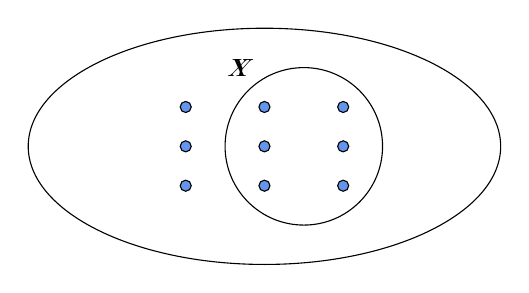
\begin{tikzpicture}[x=2cm,font=\small, fill=CornflowerBlue]
    \draw (0,0)circle (1.5) (0,1) node[ left=1.5] {$X$};
\foreach \x in {-.5,0,.5}
\foreach \y in {-.5,0,.5}
\filldraw (\x,\y) circle (2pt) node[above right] {};
\begin{scope}[y=2cm]]
    \draw (0.25,0)circle (.5) (0,.5) node[left=.1] {$Y$};
\end{scope}
\end{tikzpicture}

\end{center}
Se~$a$ è un elemento del sottoinsieme~$Y$, allora lo sarà anche dell'insieme~$X$:
\begin{center}
se~$a\in Y$ e~$Y\subseteq X$, allora~$a\in X$\qquad oppure \qquad $a\in Y$ e~$Y\subseteq X \:\Rightarrow\:a\in X$.
\end{center}

Dalla stessa definizione, si deduce che ogni insieme è sottoinsieme di
se stesso, in simboli~$X\subseteq X$.

Nel caso in cui tutti gli elementi di~$Y$ siano elementi di~$X$ e tutti gli elementi di~$X$ siano elementi di
$Y$ si ha che~$X=Y$, e~$Y$ si dice \emph{sottoinsieme improprio} di~$X$.
Se~$X\subseteq Y$ e~$Y\subseteq X$, allora~$Y=X$.

Tra i sottoinsiemi di un insieme si considera anche
l'insieme vuoto. Cioè, qualunque sia
l'insieme~$X$ risulta~$\emptyset \subseteq X$.
Quindi l'insieme vuoto è considerato un sottoinsieme improprio di qualunque insieme.

Se~$Y$ è un sottoinsieme non vuoto di~$X$ e~$X$ ha altri elementi oltre a quelli di~$Y$
si dice che~$Y$ è un \emph{sottoinsieme proprio} di~$X$ e si scrive~$Y\subset X$.

La scrittura~$Y\subseteq X$ si usa quando non si sa in modo certo se~$Y=X$ o meno.

\begin{exrig}

\begin{esempio}
Consideriamo l'insieme~$X=\{$lettere della parola ``autunno''$\}$ e
l'insieme~$Y=\{$lettere della parola ``notaio''$\}$; possiamo affermare che ogni
elemento di~$Y$ è anche elemento di~$X$? La risposta è negativa, infatti~$\text{i}\in Y$ ma
$\text{i}\notin X$ quindi~$Y$ non è sottoinsieme di~$X$ e si scrive~$Y\not\subset X$.
\end{esempio}

\begin{esempio}
Sia~$A$ l'insieme delle lettere dell'alfabeto italiano e~$V$
l'insieme delle vocali, allora si può scrivere
$V\subset A$; cioè~$V$ è un sottoinsieme proprio di~$A$,
come si può anche vedere dalla rappresentazione grafica.
\begin{center}
 % (c) 2012 Dimitrios Vrettos - d.vrettos@gmail.com
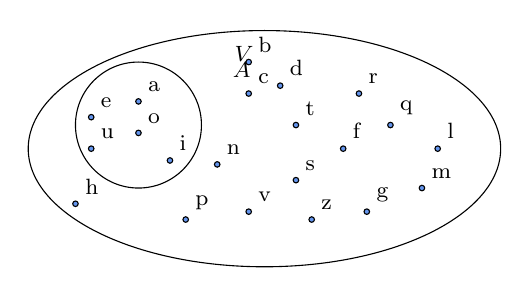
\begin{tikzpicture}[x=2cm,font=\footnotesize, fill=CornflowerBlue]
    \draw (0,0)circle (1.5) (0,1) node[ left=1.5] {$A$};
\filldraw (-.8,.6) circle (1pt) node[above right] {a};
\filldraw (-1.1,.4) circle (1pt) node[above right] {e};
\filldraw (-.6,-.15) circle (1pt) node[above right] {i};
\filldraw (-.8,.2) circle (1pt) node[above right] {o};
\filldraw (-1.1,0) circle (1pt) node[above right] {u};

\filldraw (-.1,1.1) circle (1pt) node[above right] {b};
\filldraw (-.1,.7) circle (1pt) node[above right] {c};
\filldraw (.1,.8) circle (1pt) node[above right] {d};
\filldraw (.5,0) circle (1pt) node[above right] {f};
\filldraw (.65,-.8) circle (1pt) node[above right] {g};
\filldraw (-1.2,-.7) circle (1pt) node[above right] {h};
\filldraw (1.1,0) circle (1pt) node[above right] {l};
\filldraw (1,-.5) circle (1pt) node[above right] {m};
\filldraw (-.3,-.2) circle (1pt) node[above right] {n};
\filldraw (-.5,-.9) circle (1pt) node[above right] {p};
\filldraw (.8,.3) circle (1pt) node[above right] {q};
\filldraw (.6,.7) circle (1pt) node[above right] {r};
\filldraw (.2,-.4) circle (1pt) node[above right] {s};
\filldraw (.2,.3) circle (1pt) node[above right] {t};
\filldraw (-.1,-.8) circle (1pt) node[above right] {v};
\filldraw (.3,-.9) circle (1pt) node[above right] {z};
 \begin{scope}[y=2cm]]
     \draw (-.8,.15)circle (.4) (0,.6) node[left=.4] {$V$};
 \end{scope}
\end{tikzpicture}

\end{center}
\end{esempio}

\begin{esempio}
Sia~$C=\{1\}$, allora~$C$ non ha sottoinsiemi propri;
mentre i suoi sottoinsiemi impropri sono~$C=\{1\}$ e
l'insieme vuoto~$\emptyset $.
\end{esempio}

\begin{esempio}
Sia~$A$ l'insieme delle auto esposte in un
autosalone e~$U$ l'insieme delle auto usate
esposte nello stesso autosalone. Si ha che~$U$ è un
sottoinsieme di~$A$, ma senza avere ulteriori informazioni non
possiamo escludere che tutte le auto esposte siano usate, dobbiamo
perciò scrivere~$U\subseteq A$. Se invece sappiamo che nessuna
auto esposta è usata, allora~$U=\emptyset $.
\end{esempio}
\end{exrig}

\ovalbox{\risolvii \ref{ese:7.1}, \ref{ese:7.2}, \ref{ese:7.3}, \ref{ese:7.4}, \ref{ese:7.5}, \ref{ese:7.6}}

\section{Insieme delle parti}

Consideriamo l'insieme~$A$ dei numeri naturali
compresi tra~0 e~100. A partire da questo insieme possiamo formare
gruppi costituiti dai soli numeri multipli di~10, dai numeri pari, da
quelli dispari, da quelli divisibili per~7 e così via. Quindi con gli
elementi dell'insieme~$A$ possiamo formare molti
altri insiemi che sono sottoinsiemi di~$A$.

\begin{exrig}
 \begin{esempio}
Determinare tutti i sottoinsiemi di~$A=\{$1, 2, 3$\}$.

$\emptyset \subseteq A$, infatti l'insieme vuoto è un
sottoinsieme improprio di qualunque insieme.

Elenchiamo tutti i sottoinsiemi costituiti da un solo elemento: $\{1\}$, $\{2\}$, $\{3\}$.
Elenchiamo ora tutti i sottoinsiemi costituiti da due elementi: $\{$1, 2$\}$, $\{$1, 3$\}$, $\{$2, 3$\}$.
L'unico sottoinsieme costituito da tre elementi è~$A$ stesso, possiamo scrivere:
$\{$1, 2, 3$\}\subseteq A$. In tutto si hanno 8 sottoinsiemi.
 \end{esempio}

\end{exrig}

\begin{definizione}
Dato un insieme~$A$, si chiama \emph{insieme delle parti} o (\emph{insieme potenza}) di~$A$ l'insieme $\wp(A)$ che ha come elementi
tutti i sottoinsiemi propri ed impropri di~$A$.
\end{definizione}

L'insieme delle parti di un insieme $A$ ha sempre come
elementi~$\emptyset $ e~$A$, quindi~$\emptyset\in\wp (A)$ e
$A\in\wp (A)$.
Il numero degli elementi di~$\wp (A)$, cioè dei suoi possibili
sottoinsiemi, propri e impropri, dipende dal numero degli elementi di~$A$.

\begin{exrig}
 \begin{esempio}
 L'insieme vuoto ha come unico sottoinsieme se stesso,
quindi~$\wp (\emptyset )=\{\emptyset \}$.
 \end{esempio}

\begin{esempio}
 Dato l'insieme~$A=\{a\}$, i suoi possibili sottoinsiemi
propri ed impropri sono:~$S_{1}=\emptyset$, $S_{2}=\{a\}$;
allora~$\wp (A)=\{S_{1}\text{, }S_{2}\}$.
 \end{esempio}

\begin{esempio}
 Dato l'insieme~$B=\{\text{matita, penna}\}$ i
suoi possibili sottoinsiemi propri ed impropri sono:~$S_{1}=\emptyset$,
$S_{2}=B=\{\text{matita, penna}\}$, $S_{3}=\{\text{matita}\}$,
$S_{4}=\{\text{penna}\}$;
allora~$\wp (A)=\{S_{1}\text{, }S_{2}\text{, }S_{3}\text{, }S_{4}\}$.
 \end{esempio}

\begin{esempio}
 Dato l'insieme~$B=\{\text{1, 2, 3}\}$, i suoi possibili
sottoinsiemi propri ed impropri sono:~$S_{1}=\emptyset$,
$S_{2}=B=\{\text{1, 2, 3}\}$, $S_{3}=\{1\}$, $S_{4}=\{2\}$, $S_{5}=\{3\}$,
$S_{6}=\{1\text{, }2\}$, $S_{7}=\{1\text{, }3\}$, $S_{8}=\{2\text{, }3\}$;
allora~$\wp (A)=\{S_{1}\text{, }S_{2}\text{, }S_{3}\text{, }S_{4}\text{, }S_{5}\text{, }S_{6}\text{, }S_{7}\text{, }S_{8}\}$.
 \end{esempio}
 \end{exrig}

 Riassumendo:
\begin{itemize*}
\item se~$A=\emptyset $ l'insieme delle parti ha~1 solo elemento;
\item se~$A$ ha~1 elemento allora l'insieme delle parti ha~2 elementi;
\item se~$A$ ha~2 elementi, l'insieme delle parti ne ha~4;
\item se~$A$ ha~3 elementi, l'insieme delle parti ne ha~8.
\end{itemize*}

Generalizzando, se~$A$ ha~$n$ elementi, l'insieme delle parti $\wp (A)$ ne ha~$2^{n}$.

\vspazio\ovalbox{\risolvii \ref{ese:7.7}, \ref{ese:7.8}, \ref{ese:7.9}, \ref{ese:7.10}, \ref{ese:7.11}}

\section{Insieme unione}

Prendiamo l'insieme~$P$ dei numeri pari e l'insieme~$D$ dei numeri dispari; allora
l'insieme~$\insN$ dei numeri naturali è dato dall'unione dei due insiemi~$P$ e~$D$.

\begin{definizione}
Dati due insiemi~$A$ e~$B$, si dice
\emph{insieme unione} l'insieme~$C$, composto da tutti gli elementi appartenenti ad
$A$ o a~$B$ o a entrambi.
In simboli:~$C=A\cup B$ e si legge ``$A$ unito a~$B$''
o ``$A$ unione~$B$''.
\end{definizione}
\begin{center}
 % (c) 2012 Dimitrios Vrettos - d.vrettos@gmail.com
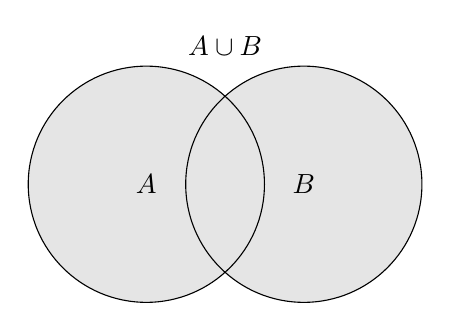
\begin{tikzpicture}[filled/.style={fill=circle area, draw=black, thin}]

\def\firstcircle{(0,0) circle (1.5cm)}
\def\secondcircle{(0:2cm) circle (1.5cm)}

\definecolor{circle area}{gray}{.9}

 \draw[filled] \firstcircle node {$A$}
                  \secondcircle node {$B$};
 \node[anchor=south] at (current bounding box.north) {$A \cup B$};
\end{tikzpicture}

\end{center}
Mediante la proprietà caratteristica si scrive:~$C=A\cup B=\{x\mid (x\in A)\text{ o }(x\in B)\}$.

\subsection{Proprietà dell'unione tra insiemi}

\begin{enumeratea}
\item $A\cup B=B\cup A$: proprietà \emph{commutativa} dell'unione;
\item $(A\cup B)\cup C=A\cup (B\cup C)$: proprietà \emph{associativa} dell'unione;
\item se~$B\subset A$, allora~$A\cup B=A$;
\item $A\cup \emptyset =A$;
\item $A\cup A=A$: proprietà di \emph{idempotenza} dell'unione;
\item $\emptyset \cup \emptyset = \emptyset $.
\end{enumeratea}
\pagebreak
\begin{exrig}
 \begin{esempio}
Siano~$D=\{$1, 3, 5$\}$ e~$P=\{$2, 4, 6$\}$ allora~$N=P\cup D=\{$1, 2, 3, 4, 5, 6$\}$.
\begin{center}
 % (c) 2012 Dimitrios Vrettos - d.vrettos@gmail.com
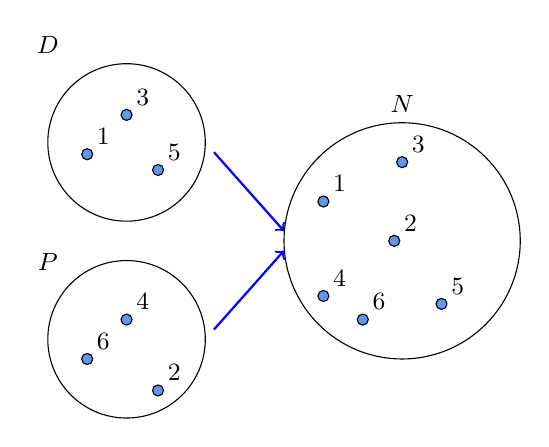
\begin{tikzpicture}[font=\small, fill=CornflowerBlue]
\draw (0,1.25)circle (1) (-1,2.25) node[above] {$D$};
\draw(0,-1.25) circle (1) (-1,-.5) node [above]  {$P$};
\draw (3.5,0) circle (1.5) (3.5,1.5) node [above]  {$N$};

\filldraw (-.5,1.1) circle (2pt) node[above right] {1};
\filldraw (0,1.6) circle (2pt) node[above right] {3};
\filldraw (.4,.9) circle (2pt) node[above right] {5};

\filldraw (-.5,-1.5) circle (2pt) node[above right] {6};
\filldraw (0,-1) circle (2pt) node[above right] {4};
\filldraw (.4,-1.9) circle (2pt) node[above right] {2};

\filldraw (2.5,.5) circle (2pt) node[above right] {1};
\filldraw (3.5,1) circle (2pt) node[above right] {3};
\filldraw (4,-.8) circle (2pt) node[above right] {5};

\filldraw (3,-1) circle (2pt) node[above right] {6};
\filldraw (2.5,-.7) circle (2pt) node[above right] {4};
\filldraw (3.4,0) circle (2pt) node[above right] {2};

\node (d) at (1,1.25) {};
\node (p) at (1,-1.25) {};
\node (n) at (2,0) {};

\begin{scope}[blue, ->,thick]
\draw (d)--(n.north);
\draw (p)--(n.south);
\end{scope}
\end{tikzpicture}

\end{center}

\end{esempio}

\begin{esempio}
Siano~$X=\{$do, re, mi, fa, sol, la, si$\}$
e~$Y=\{$do, re, mi$\}$, allora, poiché $Y\subset X$, $W=X\cup Y=X=\{$do, re, mi, fa, sol, la, si$\}$.
\begin{center}
 % (c) 2012 Dimitrios Vrettos - d.vrettos@gmail.com
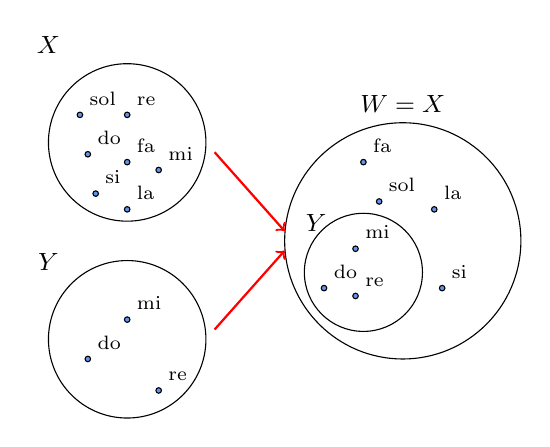
\begin{tikzpicture}[fill=CornflowerBlue]
\begin{scope}[font=\small]
\draw (0,1.25)circle (1) (-1,2.25) node[above] {$X$};
\draw(0,-1.25) circle (1) (-1,-.5) node [above]  {$Y$};
\draw (3.5,0) circle (1.5) (3.5,1.5) node [above]  {$W=X$};
\draw(3,-.4) circle (.75) (2.4,0) node [above] {$Y$};
\end{scope}
\begin{scope}[font=\scriptsize]
\filldraw (-.5,1.1) circle (1pt) node[above right] {do};
\filldraw (0,1.6) circle (1pt) node[above right] {re};
\filldraw (.4,.9) circle (1pt) node[above right] {mi};
\filldraw (0,1) circle (1pt) node[above right] {fa};
\filldraw (-.6,1.6) circle (1pt) node[above right] {sol};
\filldraw (0,.4) circle (1pt) node[above right] {la};
\filldraw (-.4,.6) circle (1pt) node[above right] {si};

\filldraw (-.5,-1.5) circle (1pt) node[above right] {do};
\filldraw (0,-1) circle (1pt) node[above right] {mi};
\filldraw (.4,-1.9) circle (1pt) node[above right] {re};

\filldraw (2.5,-.6) circle (1pt) node[above right] {do};
\filldraw (2.9,-.7) circle (1pt) node[above right] {re};
\filldraw (2.9,-.1) circle (1pt) node[above right] {mi};
\filldraw (3,1) circle (1pt) node[above right] {fa};
\filldraw (3.2,.5) circle (1pt) node[above right] {sol};
\filldraw (3.9,.4) circle (1pt) node[above right] {la};
\filldraw (4,-.6) circle (1pt) node[above right] {si};
\end{scope}
\node (x) at (1,1.25) {};
\node (y) at (1,-1.25) {};
\node (w) at (2,0) {};

\begin{scope}[red, ->,thick]
\draw (x)--(w.north);
\draw (y)--(w.south);
\end{scope}
\end{tikzpicture}

\end{center}

\end{esempio}
\end{exrig}

\ovalbox{\risolvii \ref{ese:7.12}, \ref{ese:7.13}, \ref{ese:7.14}, \ref{ese:7.15}}

\section{Insieme intersezione}

\begin{exrig}
\vspace{1.05ex}
 \begin{esempio}
Se~$A$ è l'insieme delle lettere della parola ``matematica'' e~$B$ è l'insieme delle lettere della parola
``materia''. Quali elementi di~$A$ stanno in~$B$? Quali elementi di~$B$ stanno in~$A$? Quali sono gli elementi
che stanno in entrambi gli insiemi?

\begin{itemize*}
 \item L'insieme degli elementi di~$A$ che stanno in~$B$ è $\{$m, a, t, e, i$\}$;
 \item l'insieme degli elementi di~$B$ che stanno in~$A$ è $\{$m, a, t, e, i$\}$;
 \item l'insieme degli elementi che stanno sia in~$A$ sia in~$B$ è $\{$m, a, t, e, i$\}$.
\end{itemize*}
\end{esempio}
\end{exrig}

\begin{definizione}
Dati due insiemi~$A$ e~$B$, si dice \emph{insieme intersezione} di~$A$ e~$B$, l'insieme
$C$ composto da tutti gli elementi appartenenti contemporaneamente ad
$A$ e a~$B$, ossia comuni a entrambi.
In simboli:~$C=A\cap B$, che si legge
``$A$ intersecato a~$B$'' o ``$A$ intersezione~$B$''.
\end{definizione}
\begin{center}
 % (c) 2012 Dimitrios Vrettos - d.vrettos@gmail.com
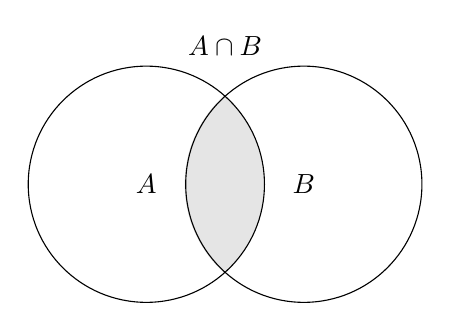
\begin{tikzpicture}[filled/.style={fill=circle area, draw=circle edge, thick}]
\def\firstcircle{(0,0) circle (1.5cm)}
\def\secondcircle{(0:2cm) circle (1.5cm)}

\definecolor{circle edge}{gray}{0.9}
\definecolor{circle area}{gray}{0.9}
    \begin{scope}
        \clip \firstcircle;
        \fill[filled] \secondcircle;
    \end{scope}
    \draw\firstcircle node {$A$};
    \draw \secondcircle node {$B$};
    \node[anchor=south] at (current bounding box.north) {$A \cap B$};
\end{tikzpicture}

\end{center}
Mediante proprietà caratteristica si scrive:~$C=A\cap B=\{x\mid (x\in A)\text{ e }(x\in B)\}$.

Se~$A$ e~$B$ non hanno elementi in comune,
ossia $A\cap B=\emptyset $, i due insiemi si dicono \emph{disgiunti}.

\subsection{Proprietà dell'intersezione tra insiemi}

\begin{enumeratea}
\item $A\cap B=B\cap A$: proprietà \emph{commutativa} dell'intersezione;
\item $(A\cap B)\cap C=A\cap (B\cap C)$: proprietà \emph{associativa} dell'intersezione;
\item Se~$B\subset A$, allora~$A\cap B=B$;
\item $A\cap \emptyset =\emptyset$;
\item $A\cap A=A$: proprietà di \emph{idempotenza} dell'intersezione;
\item $\emptyset \cap \emptyset =\emptyset$.
\end{enumeratea}

\subsection[Proprietà distributiva dell'intersezione]{Proprietà distributiva dell'intersezione rispetto all'unione e viceversa}

\begin{enumeratea}
\item $A\cap (B\cup C)=(A\cap B)\cup (A\cap C)$: proprietà \emph{distributiva dell'intersezione rispetto all'unione};
\item $A\cup (B\cap C)=(A\cup B)\cap (A\cup C)$: proprietà \emph{distributiva dell'unione rispetto all'intersezione}.
\end{enumeratea}

\begin{definizione}
Dati due insiemi si dicono \emph{disgiunti} se non hanno elementi in comune, ossia se la loro intersezione è vuota.
\end{definizione}

\begin{exrig}
 \begin{esempio}
Siano~$X=\{\text{do, re, mi. fa, sol, la, si}\}$
e~$Y=\{\text{do, re, mi}\}$. Allora poiché, 
$Y\subset X$, si ha:~$W=X\cap Y=Y=\{\text{do, re, mi}\}$.
 \end{esempio}

 \begin{esempio}
Siano~$D=\{\text{1, 3, 5}\}$ e~$P=\{\text{2, 4, 6}\}$ allora~$N=P\cap D=\emptyset$.
\begin{center}
 % (c) 2012 Dimitrios Vrettos - d.vrettos@gmail.com
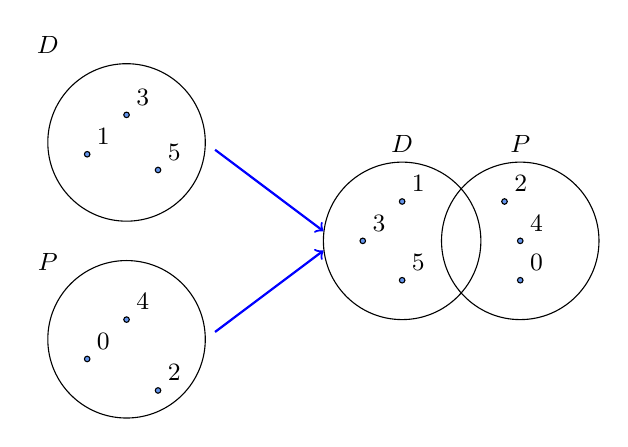
\begin{tikzpicture}[font=\small, fill=CornflowerBlue]
\draw (0,1.25)circle (1) (-1,2.25) node[above] {$D$};
\draw(0,-1.25) circle (1) (-1,-.5) node [above]  {$P$};
\draw (3.5,0) circle (1) (3.5,1) node [above]  {$D$};
\draw (5,0) circle (1) (5,1) node [above]  {$P$};

\filldraw (-.5,1.1) circle (1pt) node[above right] {1};
\filldraw (0,1.6) circle (1pt) node[above right] {3};
\filldraw (.4,.9) circle (1pt) node[above right] {5};

\filldraw (-.5,-1.5) circle (1pt) node[above right] {0};
\filldraw (0,-1) circle (1pt) node[above right] {4};
\filldraw (.4,-1.9) circle (1pt) node[above right] {2};

\filldraw (3.5,.5) circle (1pt) node[above right] {1};
\filldraw (3,0) circle (1pt) node[above right] {3};
\filldraw (3.5,-.5) circle (1pt) node[above right] {5};

\filldraw (5,-.5) circle (1pt) node[above right] {0};
\filldraw (5,0) circle (1pt) node[above right] {4};
\filldraw (4.8,.5) circle (1pt) node[above right] {2};

\node (d) at (1,1.25) {};
\node (p) at (1,-1.25) {};
\node (n) at (2.5,0) {};

\begin{scope}[blue, ->,thick]
\draw (d)--(n.north);
\draw (p)--(n.south);
\end{scope}
\end{tikzpicture}

\end{center}
 \end{esempio}
\end{exrig}

\ovalbox{\risolvii \ref{ese:7.16}, \ref{ese:7.17}, \ref{ese:7.18}, \ref{ese:7.19}}

\subsection{Insieme differenza}

Consideriamo gli insiemi~$A$ e~$B$ formati rispettivamente
dalle lettere dell'alfabeto italiano e dalle
consonanti dell'alfabeto italiano cioè:
$A=\{$a, b, c, d, e, f, g, h, i, l, m, n, o, p, q, r, s, t, u, v, z$\}$ e
$B=\{$b, c, d, f, g, h, l, m, n, p, q, r, s, t, v, z$\}$, le lettere ``a, e, i, o, u'' che compaiono
nell'insieme~$A$ ma non in~$B$ formano un nuovo insieme chiamato insieme \emph{differenza} tra $A$ e $B$.

\begin{definizione}
 Dati due insiemi~$A$ e~$B$, si dice \emph{insieme differenza} tra $A$ e $B$ l'insieme~$C$ composto da tutti gli elementi
di~$A$ che non appartengono a~$B$. In simboli:~$C=A-B$ o anche $C=A \backslash B$.
\end{definizione}

\begin{center}
% (c) 2012 Dimitrios Vrettos - d.vrettos@gmail.com
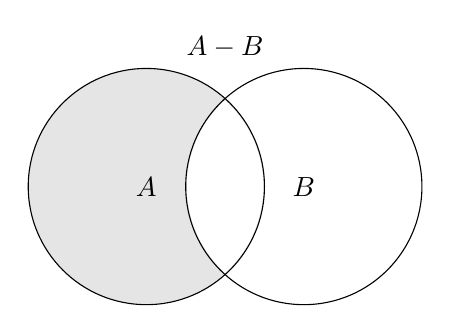
\begin{tikzpicture}[filled/.style={fill=circle area, draw=circle edge, thick}]
\def\firstcircle{(0,0) circle (1.5cm)}
\def\secondcircle{(0:2cm) circle (1.5cm)}

\definecolor{circle edge}{gray}{0.9}
\definecolor{circle area}{gray}{0.9}
\begin{scope}
\clip \firstcircle;
\draw[filled, even odd rule] \firstcircle node {$A$}
\secondcircle;
\end{scope}
\draw\firstcircle;
\draw \secondcircle node {$B$};
\node[anchor=south] at (current bounding box.north) {$A- B$};
\end{tikzpicture}

\end{center}
Mediante proprietà caratteristica si scrive:~$C=A-B=\{x\mid (x\in A)\text{ e }(x\notin B)\}$.

\subsection{Proprietà della differenza tra insiemi}

\begin{enumeratea}
\item $A-A=\emptyset$;
\item $A-\emptyset =A$;
\item se~$A\cap B=\emptyset $, ossia $A$ e $B$ sono disgiunti, allora~$A-B=A$, e~$B-A=B$;
\item se~$B\subset A$, ossia~$B$ è sottoinsieme proprio di~$A$, allora~$B-A=\emptyset $.
\end{enumeratea}

\begin{exrig}
 \begin{esempio}
Siano~$A=\{$ 8, 9, 10, 12, 13$\}$ e~$B=\{$9, 10, 11, 13$\}$, allora
$C=A-B=\{$8, 12$\}$ e~$D=B-A=\{11\}$.
 \end{esempio}
\end{exrig}

Poiché in genere $A-B\neq B-A$, nella differenza tra insiemi non vale la proprietà
commutativa.

\begin{exrig}
 \begin{esempio}
Siano~$D=\{$1, 3, 5$\}$ e~$P=\{$0, 2, 4$\}$. I due insiemi sono disgiunti poiché ~$P\cap D=\emptyset$,
 quindi~$D-P=\{$1, 3, 5$\}=D$ e~$P-D=\{$0, 2, 4$\}=P$.
\begin{center}
 % (c) 2012 Dimitrios Vrettos - d.vrettos@gmail.com
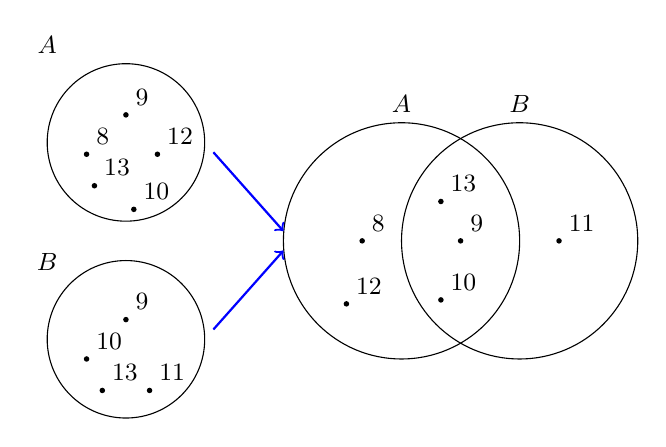
\begin{tikzpicture}[font=\small]
\draw (0,1.25)circle (1) (-1,2.25) node[above] {$A$};
\draw(0,-1.25) circle (1) (-1,-.5) node [above]  {$B$};
\draw (3.5,0) circle (1.5) (3.5,1.5) node [above]  {$A$};
\draw (5,0) circle (1.5) (5,1.5) node [above]  {$B$};

\fill (-.5,1.1) circle (1pt) node[above right] {8};
\fill (0,1.6) circle (1pt) node[above right] {9};
\fill (.4,1.1) circle (1pt) node[above right] {12};
\fill (-.4,.7) circle (1pt) node[above right] {13};
\fill (.1,.4) circle (1pt) node[above right] {10};

\fill (-.5,-1.5) circle (1pt) node[above right] {10};
\fill (0,-1) circle (1pt) node[above right] {9};
\fill (.3,-1.9) circle (1pt) node[above right] {11};
\fill (-.3,-1.9) circle (1pt) node[above right] {13};

\fill (4,.5) circle (1pt) node[above right] {13};
\fill (3,0) circle (1pt) node[above right] {8};
\fill (2.8,-.8) circle (1pt) node[above right] {12};

\fill (4,-.75) circle (1pt) node[above right] {10};
\fill (4.25,0) circle (1pt) node[above right] {9};
\fill (5.5,0) circle (1pt) node[above right] {11};

\node (a) at (1,1.25) {};
\node (b) at (1,-1.25) {};
\node (n) at (2,0) {};

\begin{scope}[blue, ->,thick]
\draw (a)--(n.north);
\draw (b)--(n.south);
\end{scope}
\end{tikzpicture}

\end{center}
 \end{esempio}

 \begin{esempio}
Siano~$X=\{$do, re, mi, fa, sol, la, si$\}$
e~$Y=\{$do, re, mi$\}$ allora poiché
$Y\subset X$, $W=X-Y=\{$fa, sol, la, si$\}$.
\begin{center}
 % (c) 2012 Dimitrios Vrettos - d.vrettos@gmail.com
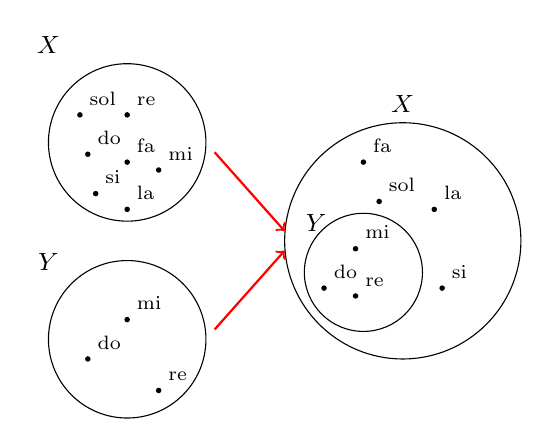
\begin{tikzpicture}
\begin{scope}[font=\small]
\draw (0,1.25)circle (1) (-1,2.25) node[above] {$X$};
\draw(0,-1.25) circle (1) (-1,-.5) node [above]  {$Y$};
\draw (3.5,0) circle (1.5) (3.5,1.5) node [above]  {$X$};
\draw(3,-.4) circle (.75) (2.4,0) node [above] {$Y$};
\end{scope}
\begin{scope}[font=\scriptsize]
\fill (-.5,1.1) circle (1pt) node[above right] {do};
\fill (0,1.6) circle (1pt) node[above right] {re};
\fill (.4,.9) circle (1pt) node[above right] {mi};
\fill (0,1) circle (1pt) node[above right] {fa};
\fill (-.6,1.6) circle (1pt) node[above right] {sol};
\fill (0,.4) circle (1pt) node[above right] {la};
\fill (-.4,.6) circle (1pt) node[above right] {si};

\fill (-.5,-1.5) circle (1pt) node[above right] {do};
\fill (0,-1) circle (1pt) node[above right] {mi};
\fill (.4,-1.9) circle (1pt) node[above right] {re};

\fill (2.5,-.6) circle (1pt) node[above right] {do};
\fill (2.9,-.7) circle (1pt) node[above right] {re};
\fill (2.9,-.1) circle (1pt) node[above right] {mi};
\fill (3,1) circle (1pt) node[above right] {fa};
\fill (3.2,.5) circle (1pt) node[above right] {sol};
\fill (3.9,.4) circle (1pt) node[above right] {la};
\fill (4,-.6) circle (1pt) node[above right] {si};
\end{scope}
\node (x) at (1,1.25) {};
\node (y) at (1,-1.25) {};
\node (w) at (2,0) {};

\begin{scope}[red, ->,thick]
\draw (x)--(w.north);
\draw (y)--(w.south);
\end{scope}
\end{tikzpicture}

\end{center}
 \end{esempio}
\end{exrig}

\ovalbox{\risolvii \ref{ese:7.20}, \ref{ese:7.21}, \ref{ese:7.22}}

\section{Insieme complementare}

Sia~$W=\{\text{sabato, domenica}\}$ l'insieme dei giorni della settimana che non finiscono per ``dì''.
L'insieme~$W$ può essere considerato come sottoinsieme dell'insieme~$G$ formato da tutti i giorni della settimana
$G=\{\text{lunedì, martedì, mercoledì, giovedì, venerdì, sabato, domenica}\}$.
L'insieme degli elementi di~$G$ che non appartengono a~$W$ forma
un insieme che chiameremo \emph{complementare} di~$W$ rispetto a~$G$. L'insieme~$G$ invece si dice, in questo caso, insieme \emph{universo}. Ad esempio
nella rappresentazione caratteristica~$A=\{x\in\insN\mid x\le~100\}$,
$\insN$ è l'insieme universo di~$A$.

\begin{definizione}
Dato un insieme~$A$, uno dei possibili insiemi che
contengono~$A$ come sottoinsieme si dice
\emph{insieme universo} o \emph{insieme ambiente}.
\end{definizione}

\begin{definizione}
Dato l'insieme~$A$ e scelto~$U$ come suo insieme universo, l'insieme degli elementi di
$U$ che non appartengono ad~$A$ è detto \emph{insieme complementare} di~$A$ rispetto a~$U$ e si indica con~$\overline{A}$ oppure~$\overline{A}_{U}$
o ancora~$\complement_{U}A$.
\end{definizione}

\begin{multicols}{2}
Il diagramma di Eulero-Venn dell'insieme $A$ e del suo universo $U$ è quello rappresentato in figura.
La parte in grigio è il complementare di~$A$ rispetto a~$U$, cioè~${\overline{A}}_{U}$.
Si può osservare che, essendo~$A\subseteq U$, il complementare coincide con la differenza tra insiemi:
${\overline{A}}_{U}=U-A$.
\begin{center}
% (c) 2012 Dimitrios Vrettos - d.vrettos@gmail.com
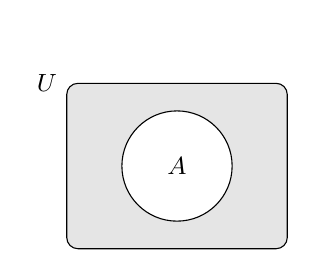
\begin{tikzpicture}[x=7mm,y=7mm,font=\small]
\definecolor{circle area}{gray}{0.9}
\draw[rounded corners, fill=circle area] (0,0) rectangle (4,3) (0,4);
\draw[fill=white](2,1.5) circle (1) (2,1.5) node {$A$};
\node [above, left] at (0,3) {$U$};
\end{tikzpicture}

\end{center}
\end{multicols}

\begin{exrig}
 \begin{esempio}
 Insiemi complementari.
\begin{enumeratea}
\item Il complementare dell'insieme~$D$ dei numeri dispari rispetto all'insieme~$\insN$ dei numeri naturali è
l'insieme~$P$ dei numeri pari:~${\overline{D}}_{\insN}=P$;
\item Il complementare dell'insieme~$V$ delle vocali dell'alfabeto italiano rispetto
all'insieme~$A$ delle lettere dell'alfabeto italiano è l'insieme~$C$ delle consonanti:
${\overline{V}}_{U}=C$;
\item Dati gli insiemi~$U=\{x\in \insN\mid 1\le x\le~10\}$ e~$B=\{x\in \insN\mid 1\le x\le~5\}$, poiché $B\subset U$
si può determinare~${\overline{B}}_{U}=\{x\in \insN\mid 6\le x\le~10\}$.
\end{enumeratea}
 \end{esempio}
\end{exrig}

\ovalbox{\risolvii \ref{ese:7.23}, \ref{ese:7.24}, \ref{ese:7.25}, \ref{ese:7.26}, \ref{ese:7.27}}

\section{Leggi di De Morgan}

Dati due insiemi~$A$ e~$B$ ci sono alcune proprietà,
dette \emph{leggi di De Morgan}\footnote{dal nome del matematico e logico britannico Augustus De Morgan (1806 - 1871).}, che semplificano lo svolgimento di alcune operazioni:

\begin{enumeratea}
\item $\overline{A\cap B}=\overline{A}\cup \overline{B}$: \emph{Prima legge di De Morgan};
\item $\overline{A\cup B}=\overline{A}\cap \overline{B}$: \emph{Seconda legge di De Morgan}.
\end{enumeratea}

Dimostriamo la prima legge di De Morgan utilizzando i diagrammi di Eulero-Venn.
\begin{center}
 % (c) 2012 Dimitrios Vrettos - d.vrettos@gmail.com
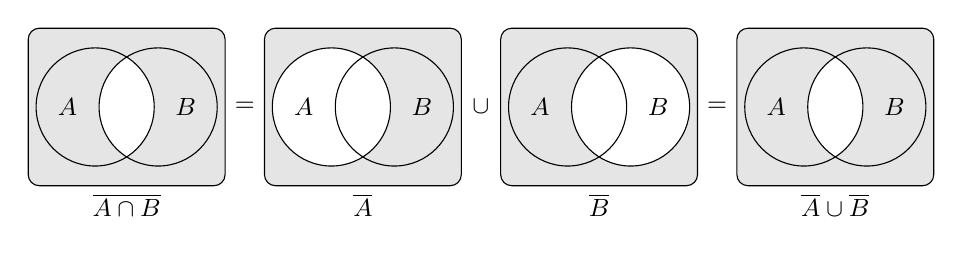
\begin{tikzpicture}[x=5mm,y=5mm,font=\small, outline/.style={draw=circle edge}]
\definecolor{circle area}{gray}{0.9}
\definecolor{circle edge}{rgb}{0,0,0}

\def\firstcircle{(1.7,2) circle (1.5)}
\def\secondcircle{(3.3,2) circle (1.5)}

\begin{scope}[rounded corners]
\foreach \i in {0,6,12,18}
\draw[fill=circle area] (\i,0) rectangle (\i+5,4);
\end{scope}

\begin{scope}]
\begin{scope}
\clip \firstcircle;
\fill[white] \secondcircle;
\end{scope}
\draw[outline] \firstcircle;
\draw[outline] \secondcircle;
\end{scope}

\begin{scope}[xshift=30mm]
\begin{scope}
\clip \firstcircle;
\fill[white] \firstcircle;
\end{scope}
 \draw[outline]  \firstcircle;
\draw[outline] \secondcircle;
\end{scope}

\begin{scope}[xshift=60mm]
\begin{scope}
\clip \secondcircle;
\fill[white] \secondcircle;
\end{scope}
 \draw[outline]  \firstcircle;
\draw[outline] \secondcircle;
\end{scope}

\begin{scope}[xshift=90mm]
\begin{scope}
\clip \firstcircle;
\fill[white] \secondcircle;
\end{scope}
\draw[outline] \firstcircle;
 \draw[outline] \secondcircle;
\end{scope}

\foreach \x/\xtext in {5.5/$=$,11.5/$\cup$,17.5/$=$}
	\node  at (\x,2) {\xtext};

\foreach \y in {1,7,13,19}
\node  at (\y,2) {$A$};

\foreach \z in {4,10,16,22}
\node  at (\z,2) {$B$};

\foreach \j/\jtext in {2.5/\overline{A\cap B},8.5/\overline{A},14.5/\overline{B},20.5/\overline{A}\cup\overline{B}
}
\node  at (\j,-.5) {$\jtext$};
\end{tikzpicture}

\end{center}

\ovalbox{\risolvi \ref{ese:7.27}}

\section{Partizione di un insieme}
\begin{definizione}
Dato un insieme~$A$ e alcuni suoi sottoinsiemi $A_1, A_2, A_3, \ldots, A_n$, si dice che costituiscono una \emph{partizione} di~$A$ se:
\begin{enumeratea}
 \item sono tutti non vuoti;
 \item sono a due a due disgiunti;
 \item la loro unione dà l'insieme~$A$.
\end{enumeratea}
\end{definizione}

\begin{exrig}
 \begin{esempio}
 Partizione di un insieme.

Dato l'insieme~$C$ delle carte da gioco napoletane, i sottoinsiemi~$A_1$ delle carte a denari, $A_2$ delle carte a spade, $A_3$ delle carte a coppe, $A_4$ delle carte a bastoni costituiscono una partizione di~$C$.

Infatti nessuno degli insiemi $A_1, A_2, A_3, A_4$ è vuoto, ciascuno è costituito da~10 elementi. Inoltre i sottoinsiemi sono a due a due disgiunti perché non ci sono carte che appartengono a $A_1 \cap A_2$, $A_1 \cap A_3$, $A_1 \cap A_4$, $A_2 \cap A_3$, $A_2 \cap A_4$, $A_3 \cap A_4$, cioè non ci sono carte che possono appartenere contemporaneamente a due semi distinti. Infine l'unione $A_1\cup A_2 \cup A_3 \cup A_4$ dà l'insieme delle carte~$C$.
 \end{esempio}
\end{exrig}

\ovalbox{\risolvii \ref{ese:7.28}, \ref{ese:7.29}, \ref{ese:7.30}, \ref{ese:7.31}}

\section{Prodotto cartesiano fra insiemi}

Supponiamo che la partita di calcio Lecce~-~Juventus sia terminata~3-2; in questo caso il risultato della partita
non rappresenta un insieme di numeri dato che nella rappresentazione di un insieme scrivere~$\{$3, 2$\}$ e~$\{$2, 3$\}$
 è la stessa cosa. Infatti, se avessimo scritto~2-3 al posto di~3-2 la partita avrebbe avuto un esito
differente. Ci troviamo nel caso di una \emph{coppia ordinata} di numeri.\footnote{si veda anche la sezione~\ref{sect:coordinate_cartesiane} a pagina~\pageref{sect:coordinate_cartesiane}.}

\begin{definizione}
Un insieme di due elementi~$a$ e~$b$
presi in un determinato ordine si dice \emph{coppia ordinata}. Se il primo elemento della coppia è
$a$ e il secondo è~$b$ si scrive:~$(a;b)$.
\end{definizione}

\begin{definizione}
Dati due insiemi~$A$ e~$B$ non vuoti,
l'insieme formato da tutte le coppie ordinate tali che
il primo elemento appartiene ad~$A$ e il secondo a~$B$, si chiama
\emph{prodotto cartesiano} di~$A$ per~$B$. In simboli:~$A\times B$ che si legge ``$A$ per~$B$''
oppure ``$A$ prodotto cartesiano con~$B$'' o ancora ``$A$ cartesiano~$B$''.
\end{definizione}

Mediante proprietà caratteristica si scrive:
$A\times B=\{(x;y)\mid x\in A\text{ e }y\in B\}$.
Nel caso in cui~$B=A$, il prodotto cartesiano diventa $A\times A=A^{2}=\{(x;y)\mid x\in A\text{ e }y\in A\}$.

\begin{exrig}
 \begin{esempio}
Sia~$C=\{x\text{, }y\text{, }z\}$, il prodotto cartesiano~$C\times C$ è dato dalle
seguenti coppie ordinate:~$C\times C=\{(x;x)\text{, }(x;y)\text{, }(x;z)\text{, }(y;x)\text{, }(y;y)\text{, }(y;z)\text{, }(z;x)\text{, }(z;y)\text{, }(z;z)\}$.
 \end{esempio}
\end{exrig}

\subsection{Proprietà del prodotto cartesiano tra insiemi}

\begin{enumeratea}
 \item $A\times \emptyset =\emptyset$;
 \item $\emptyset \times A=\emptyset$;
 \item $\emptyset \times \emptyset =\emptyset$.
\end{enumeratea}

\begin{exrig}
 \begin{esempio}
Sia~$A=\{\text{a, b}\}$ e~$B=\{\text{1, 2, 3}\}$. Il prodotto cartesiano~$A\times B$ è dato dalle seguenti coppie ordinate:
$A\times B=\{(\text{a};1)\text{, }(\text{a};2)\text{, }(\text{a};3)\text{, }(\text{b};1)\text{, }(\text{b};2)\text{, }(\text{b};3)\}$, mentre il prodotto cartesiano~$B\times A$
è dato dalle seguenti coppie ordinate:
$B\times A=\{(1;\text{a})\text{, }(2;\text{a})\text{, }(3;\text{a})\text{, }(1;\text{b})\text{, }(2;\text{b})\text{, }(3;\text{b})\}$.
Quindi si può notare che~$A\times B\neq B\times A$.
 \end{esempio}
\end{exrig}

Poiché $A\times B\neq B\times A$ nel prodotto cartesiano non vale la
proprietà commutativa.

\vspazio\ovalbox{\risolvii \ref{ese:7.32}, \ref{ese:7.33}, \ref{ese:7.34}, \ref{ese:7.35}, \ref{ese:7.36}, \ref{ese:7.37}}

\subsection{Rappresentazione del prodotto cartesiano tra insiemi}
\paragraph{Tabulazione delle coppie ordinate}

Come fatto nei precedenti esempi, si combina il primo elemento
di~$A$ con tutti gli elementi di~$B$, il secondo elemento
di~$A$ con tutti gli elementi di~$B$ e cosi via fino ad
esaurire tutti gli elementi di~$A$.
\[A\times B=\{(\text{a};1)\text{, }(\text{a};2)\text{, }(\text{a};3)\text{, }(\text{b};1)\text{, }(\text{b};2)\text{, }(\text{b};3)\}.\]

\paragraph{Diagramma a frecce}
Si rappresentano i due insiemi graficamente
con i diagrammi di Eulero-Venn e si tracciano degli archi orientati che
escono dagli elementi del primo insieme e raggiungono gli elementi del
secondo insieme formando coppie ordinate del prodotto cartesiano.
\begin{center}
% (c) 2012 Dimitrios Vrettos - d.vrettos@gmail.com
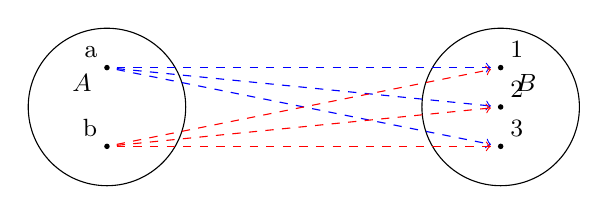
\begin{tikzpicture}[x=5mm,y=5mm,font=\small]

\def\firstcircle{(0,0) circle (2)}
\def\secondcircle{(10,0) circle (2)}

\draw \firstcircle node [above left=2]  {$A$};
\draw \secondcircle node [above right=2]  {$B$};

\fill (0,1) circle (1pt) node[above left] {a};
\fill (0,-1) circle (1pt) node[above left](b) {b};

\fill (10,1) circle (1pt) node[above right] {1};
\fill (10,0) circle (1pt) node[above right] {2};
\fill (10,-1) circle (1pt) node[above right] {3};

\node (a) at (0,1) {};
\node (b) at (0,-1) {};
\node (uno) at (10,1) {};
\node (due) at (10,0) {};
\node (tre) at (10,-1) {};
\begin{scope}[->,dashed]
\begin{scope}[blue]
\draw (a) -- (uno);
\draw (a) -- (due);
\draw (a) -- (tre);
\end{scope}
\begin{scope}[red]
\draw (b) -- (uno);
\draw (b) -- (due);
\draw (b) -- (tre);
\end{scope}
\end{scope}
\end{tikzpicture}

\end{center}

\paragraph{Tabella a doppia entrata}

Si costruisce una tabella nella quale si riportano gli elementi del
primo insieme sulla prima colonna e gli elementi del secondo insieme
sulla prima riga. Le caselle di incrocio rappresentano le coppie
ordinate del prodotto cartesiano.
\begin{center}
 % (c) 2012 Dimitrios Vrettos - d.vrettos@gmail.com
\begin{tikzpicture}[font=\small]

\matrix(m) [matrix of nodes, nodes={minimum size=7mm}]{
{}& 1 & 2 & 3\\
a & $(\text{a};1)$& $(\text{a};2)$& $(\text{a};3)$\\
b & $(\text{b};1)$& $(\text{b};2)$& $(\text{b};3)$\\
};
\draw (m-2-1.north west)--(m-2-4.north east);
\draw (m-1-1.north east)--(m-3-1.south east);

\draw[decoration=brace,decorate] (m-1-2.north)--(m-1-4.north) node[above, midway] {$B$};
\draw[decoration={brace,mirror}, decorate] (m-2-1.west)--(m-3-1.west) node[left, midway] {$A$};

\end{tikzpicture}

\end{center}

\begin{wrapfloat}{figure}{r}{0pt}
 % (c) 2012 Dimitrios Vrettos - d.vrettos@gmail.com
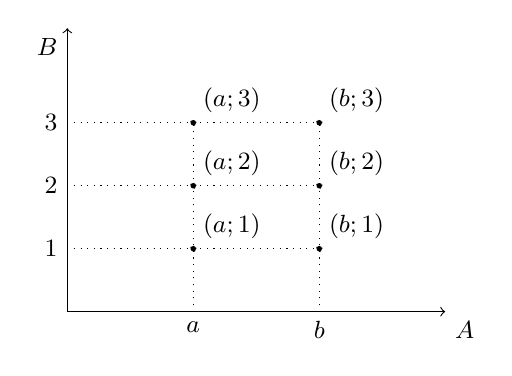
\begin{tikzpicture}[x=16mm, y=8mm,font=\small]
\draw[->] (0,0)--(3,0) node [below right]{$A$};
\draw[->] (0,0)--(0,4.5) node [below left]{$B$};

\begin{scope}[dotted]
\foreach \x in {1,2}
\foreach \y in {1,2,3}{
\draw (\x,0) -- (\x,\y);
\draw (0,\y) -- (\x,\y);
\draw[fill](\x,\y) circle (1pt);
}
\end{scope}

\begin{scope}[above right]
\node at (1,1) {$(\text{a};1)$};
\node at (1,2) {$(\text{a};2)$};
\node at (1,3) {$(\text{a};3)$};
\node at (2,1) {$(\text{b};1)$};
\node at (2,2) {$(\text{b};2)$};
\node at (2,3) {$(\text{b};3)$};
\end{scope}

\foreach \xi/\xitext in {1/$\text{a}$,2/$\text{b}$}
\node[below] at (\xi,0) {\xitext};

\foreach \yi/\yitext in {1/1,2/2,3/3}
\node[left] at (0,\yi) {\yitext};

\end{tikzpicture}

\end{wrapfloat}

\paragraph{Diagramma cartesiano}
Si tracciano due semirette orientate, perpendicolari, una orizzontale e l'altra
verticale, con l'origine
in comune. Si riportano gli elementi del primo insieme sulla semiretta
orizzontale e quelli del secondo su quella verticale. Tali semirette
vengono chiamate \emph{assi cartesiani}. Si tracciano prima le
parallele all'asse verticale dai punti individuati
sull'asse orizzontale che rappresentano gli elementi
del primo insieme, poi le parallele all'asse
orizzontale dai punti sull'asse verticale; i punti di
intersezione rappresentano le coppie ordinate del prodotto
cartesiano.

\paragraph{Diagramma ad albero}
\`E un grafico formato da un nodo iniziale dal quale si ripartono alcuni
rami che a loro volta possono ramificarsi e così via fino a che nello
schema figurano tutte le possibili situazioni.
Si può raggiungere un particolare nodo solo muovendosi lungo i rami ed
il percorso che collega due nodi qualsiasi deve essere unico.

La rappresentazione mediante diagramma ad albero è vantaggiosa nel
caso si voglia fare il prodotto cartesiano tra più insiemi.
\begin{center}
% (c) 2012 Dimitrios Vrettos - d.vrettos@gmail.com
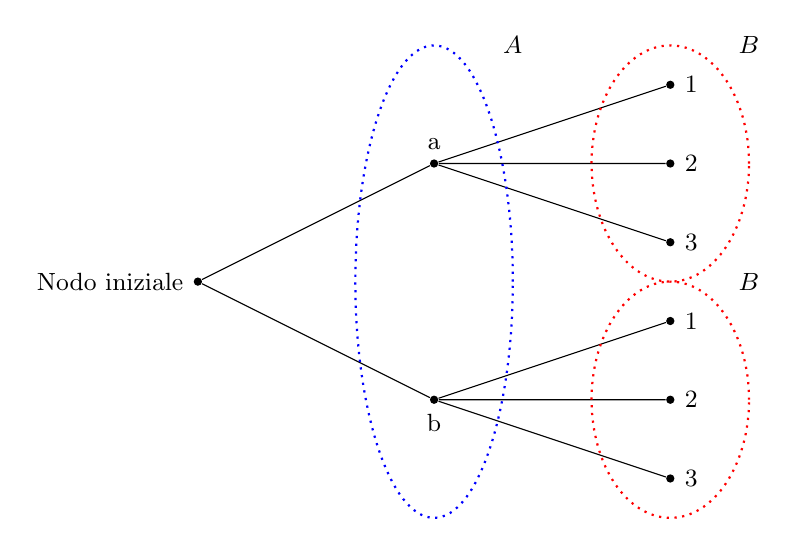
\begin{tikzpicture}[x=5mm, y=5mm,font=\small]
\tikzstyle{level 1}=[level distance=3cm, sibling distance=3cm]
\tikzstyle{level 2}=[level distance=3cm, sibling distance=1cm]
\tikzstyle{point} = [circle,minimum width=3pt,fill, inner sep=0pt]

\node[point, label=left:{Nodo iniziale}] (aer) at (0,0) {}[grow'=right]
child {node[point, label=above:{a}] {} 
child {node[point,label=right:{1}] {}}
child {node[point,label=right:{2}] {}}
child {node[point,label=right:{3}] {}}
}
child {node[point, label=below:{b}] {} 
child {node[point,label=right:{1}] {}}
child {node[point,label=right:{2}] {}}
child {node[point,label=right:{3}] {}}
} ;

\begin{scope}[dotted,thick]
\draw[blue] (6,0) ellipse (2 and 6)  (8,6)node [black] {$A$};
\draw[red] (12,3) ellipse (2 and 3) (14,6)node [black] {$B$};
\draw[red] (12,-3) ellipse (2 and 3)  (14,0)node [black] {$B$};

\end{scope}
\end{tikzpicture}

\end{center}

\begin{exrig}
 \begin{esempio}
 Una compagnia aerea deve organizzare delle rotte per collegare fra loro alcune città effettuando uno scalo
in un'altra città. Sia~$P=\{$Brindisi, Bari, Palermo$\}$ l'insieme delle città di
partenza, $S=\{$Roma, Milano$\}$ l'insieme delle città di
scalo e~$A=\{$Parigi, Berlino, Londra$\}$ l'insieme delle città di
arrivo. Per conoscere tutte le possibili rotte aeree dobbiamo
determinare il prodotto cartesiano tra i~3 insiemi~$P\times S\times A$.
Rappresentiamo~$P\times S\times A$ tramite un diagramma ad albero:
%\newpage
\begin{center}
% (c) 2012 Dimitrios Vrettos - d.vrettos@gmail.com
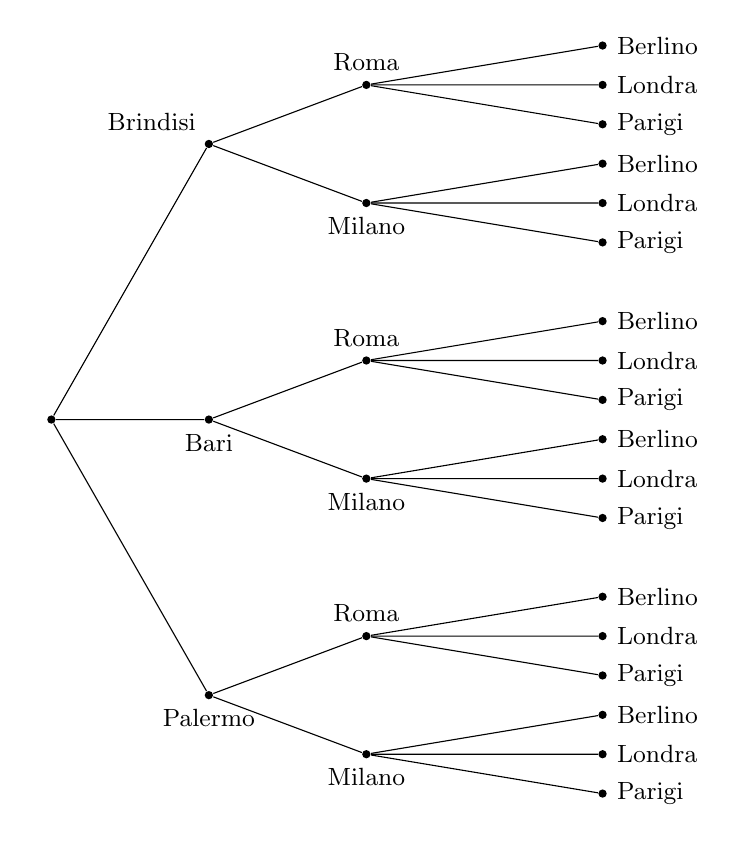
\begin{tikzpicture}[x=5mm, y=5mm,font=\small]
\tikzstyle{level 1}=[level distance=2cm, sibling distance=3.5cm]
\tikzstyle{level 2}=[level distance=2cm, sibling distance=1.5cm]
\tikzstyle{level 3}=[level distance=3cm, sibling distance=.5cm]
\tikzstyle{point} = [circle,minimum width=3pt,fill, inner sep=0pt]

\node[point, label=left:{}] (aer) at (0,0) {}[grow'=right]
  child {node[point, label=above left:{Brindisi}] {} 
    child {node[point,label=above:{Roma}] {}
      child {node[point, label=right:{Berlino}] {}}
      child {node[point, label=right:{Londra}] {}}
      child {node[point, label=right:{Parigi}] {}}
    }
    child {node[point,label=below:{Milano}] {}
      child {node[point, label=right:{Berlino}] {}}
      child {node[point, label=right:{Londra}] {}}
      child {node[point, label=right:{Parigi}] {}}}
    }
  child {node[point, label=below:{Bari}] {} 
    child {node[point,label=above:{Roma}] {}
      child {node[point, label=right:{Berlino}] {}}
      child {node[point, label=right:{Londra}] {}}
      child {node[point, label=right:{Parigi}] {}}}
    child {node[point,label=below:{Milano}] {}
      child {node[point, label=right:{Berlino}] {}}
      child {node[point, label=right:{Londra}] {}}
      child {node[point, label=right:{Parigi}] {}}}
    }
  child {node[point, label=below:{Palermo}] {} 
    child {node[point,label=above:{Roma}] {}
      child {node[point, label=right:{Berlino}] {}}
      child {node[point, label=right:{Londra}] {}}
      child {node[point, label=right:{Parigi}] {}}}
    child {node[point,label=below:{Milano}] {}
      child {node[point, label=right:{Berlino}] {}}
      child {node[point, label=right:{Londra}] {}}
      child {node[point, label=right:{Parigi}] {}}}
};
\end{tikzpicture}

\end{center}
 \end{esempio}
\end{exrig}

\section{I diagrammi di Eulero-Venn come modello di un problema}
Alcune volte, trovandoci di fronte a un problema, possiamo rappresentare
la situazione con diagrammi di Eulero-Venn, ciò agevola la
comprensione e facilita la risoluzione del problema. Attraverso alcuni
esempi mostreremo come usare la teoria degli insiemi per risolvere
problemi.

\begin{exrig}
 \begin{esempio}
Nel seguente diagramma di Eulero-Venn, l'insieme~$A$ rappresenta un gruppo di amici appassionati di ballo; gli insiemi~$T$, $R$,
$S$ rappresentano rispettivamente coloro che ballano il tango, la rumba, il samba; ogni puntino rappresenta uno degli amici.
\begin{multicols}{2}
Quanti sono gli amici appassionati di ballo?

Quanti tra loro ballano:
\begin{enumeratea}
\item \emph{nessuno} dei balli indicati?
\item \emph{almeno uno} dei balli tango, samba, rumba?
\item \emph{almeno} il samba?
\item \emph{solo} la rumba?
\item la rumba \emph{e} il tango?
\item \emph{tutti} i balli indicati?
\end{enumeratea}
\begin{center}
 % (c) 2012 Dimitrios Vrettos - d.vrettos@gmail.com
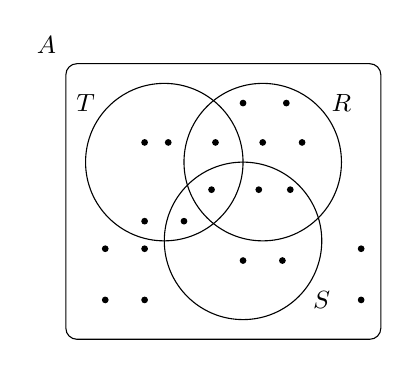
\begin{tikzpicture}[x=5mm, y=5mm,font=\small]

\draw[rounded corners] (0,0) rectangle (8,7) (0,7) node [above left]  {$A$};
\draw (2.5,4.5) circle (2) (.5,6)node {$T$};
\draw (5,4.5) circle (2) (7,6)node {$R$};
\draw (4.5,2.5) circle (2) (6.5,1)node {$S$};

\foreach \x in {2,2.6,3.8,5,6}
\draw[fill] (\x,5) circle (1pt);

\foreach \xi in {4.5,5.6}
\draw[fill] (\xi,6) circle (1pt);

\foreach \xii in {3.7,4.9,5.7}
\draw[fill] (\xii,3.8) circle (1pt);

\foreach \xiii in {2,3}
\draw[fill] (\xiii,3) circle (1pt);

\foreach \xiv in {4.5,5.5}
\draw[fill] (\xiv,2) circle (1pt);

\foreach \xv in {1,2,7.5}{
\draw[fill] (\xv,1) circle (1pt);
\draw[fill] (\xv,2.3) circle (1pt);
}
\end{tikzpicture}

\end{center}
\end{multicols}

Per rispondere alle domande dobbiamo contare gli elementi che formano determinati insiemi.

Quanti sono gli amici appassionati di ballo? Per rispondere a questa
domanda, contiamo tutti i puntini che compaiono nel disegno. Si ha 
$\card(A)=20$.

Rispondiamo ora alle altre domande.
\begin{enumeratea}
\item Quanti tra loro ballano \emph{nessuno} dei balli indicati?
Chi non balla nessuno dei balli indicati sta nell'insieme~$A$, ma in nessuno degli insiemi
$R$, $S$, $T$ quindi appartiene al complementare
di~$R\cup S\cup T$ rispetto all'insieme~$A$,
dunque~$\card(\overline{({R\cup S\cup T})}_{A})=6$.

\item Quanti tra loro ballano \emph{almeno uno} dei balli tra tango, samba, rumba? Chi balla almeno uno di quei balli è rappresentato dagli elementi
dell'insieme~$R\cup S\cup T$, quindi~$\card(R\cup S\cup T)=14$.

\item Quanti tra loro ballano \emph{almeno} il samba?
Gli amici che ballano almeno il samba sono nell'insieme
$S$, quindi~$\card(S)=6$.

\item Quanti tra loro ballano \emph{solo} la rumba? Nell'insieme~$R$ sono rappresentati gli amici che
ballano almeno il rumba, quindi dobbiamo togliere dall'insieme~$R$ gli elementi che stanno in
$S$ o in~$T$:~$\card(R-(T\cup S))=4$.

\item Quanti tra loro ballano la rumba \emph{e} il tango? Quelli che ballano sia la rumba che il tango sono gli elementi
dell'insieme intersezione~$R\cap T$, quindi~$\card(R\cap T)=2$.

\item Quanti tra loro ballano \emph{tutti} i balli indicati? Quelli che ballano tutti e tre i balli indicati sono elementi
dell'insieme intersezione~$R\cap S\cap T$, quindi~$\card(R\cap S\cap T)=1$.
\end{enumeratea}
 \end{esempio}

 \begin{esempio}
 A settembre, per la festa delle contrade, a Lainate è arrivato un luna
park dove, oltre ad una grande giostra, era stato allestito un tiro a
segno con palline di gommapiuma, proprio per i bambini. Alcuni
bambini, accompagnati dalla loro maestra si sono recati al luna park: 7
sono stati sulla giostra, 3 sono stati sia sulla giostra che al tiro a
segno, 3 si sono divertiti solamente col tiro a segno e altri~2 sono
stati a guardare. Quanti bambini sono andati quel giorno al luna park?

\begin{multicols}{2}
Per risolvere il problema rappresentiamo con diagrammi di Eulero-Venn la situazione; indichiamo con~$B$ l'insieme dei
bambini recatisi al luna park, con~$G$ l'insieme di quelli che sono stati sulla giostra e con~$T$ l'insieme
di quelli che hanno provato il tiro a segno.
Dall'enunciato sappiamo che~$\card(G)=7$, $\card(G\cap T)=3$, $\card(T-G)=3$ e~$\card(B-(G\cup T))=2$.
\begin{center}
 % (c) 2012 Dimitrios Vrettos - d.vrettos@gmail.com
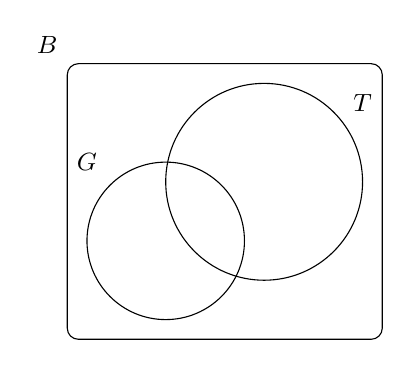
\begin{tikzpicture}[x=5mm, y=5mm,font=\small]

\draw[rounded corners] (0,0) rectangle (8,7) (0,7) node [above left]  {$B$};
\draw (2.5,2.5) circle (2) (.5,4.5)node {$G$};
\draw (5,4) circle (2.5) (7.5,6)node {$T$};

\end{tikzpicture}

\end{center}
\end{multicols}

Completa la rappresentazione segnando i bambini con dei puntini e rispondi al quesito.
\end{esempio}

\begin{esempio}
Alla palestra Anni Verdi, il giovedì si tengono due allenamenti di pallavolo e calcio dalle~17.00 alle~18.30. Frequentano il corso di
pallavolo~15 persone e sono~28 quelli che frequentano l'allenamento di calcio. Quante persone frequentano
pallavolo o calcio in questo orario?
\paragraph{Dati} $P=\{$iscritti a pallavolo$\}$, $C=\{$iscritti a calcio$\}$, $\card(P)=15$, $\card(C)=28$.
\paragraph{Obiettivo} Il problema chiede di determinare la cardinalità di~$P\cup C$.
%\begin{multicols}{2}
\paragraph{Soluzione} Osserviamo che non ci sono persone che frequentano sia
l'uno che l'altro sport essendo gli allenamenti nello stesso orario; gli insiemi~$P$ e~$C$
sono disgiunti:~$P\cap C=\emptyset $. Quindi:~$\card(P\cup C)=\card(P)+\card(C)=15+28=43$.

% \begin{center}
% % (c) 2012 Dimitrios Vrettos - d.vrettos@gmail.com
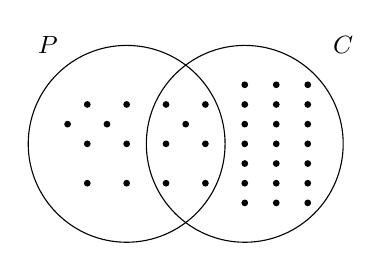
\begin{tikzpicture}[x=5mm, y=5mm,font=\small]

\draw (2,0) circle (2.5) (0,2.5)node {$P$};
\draw (5,0) circle (2.5) (7.5,2.5)node {$C$};

\foreach \x in {1,2,3,4}
\foreach \y in {-1,0,1}
\draw[fill] (\x,\y) circle (1pt);

\foreach \z in {.5,1.5,3.5}
\draw[fill] (\z,.5) circle (1pt);

\foreach \i in {5,5.8,6.6}
\foreach \j in {1.5,1,.5,0,-.5,-1,-1.5}
\draw[fill] (\i,\j) circle (1pt); 
\end{tikzpicture}

% \end{center}
%\end{multicols}
\end{esempio}

\begin{esempio}
\begin{multicols}{2}
 Alla palestra Anni Verdi, il lunedì si tengono allenamenti di pallavolo dalle~17.00 alle~18.30 e dalle~19.00 alle~20.30 gli
allenamenti di calcio. Quelli che frequentano la pallavolo sono~15, quelli che frequentano il calcio sono~28, però ce ne sono~7 di loro
che fanno entrambi gli allenamenti. Quanti sono gli sportivi che si allenano il lunedì?
\begin{center}
 % (c) 2012 Dimitrios Vrettos - d.vrettos@gmail.com
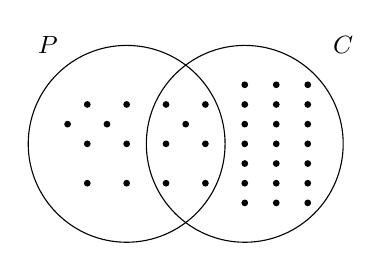
\begin{tikzpicture}[x=5mm, y=5mm,font=\small]

\draw (2,0) circle (2.5) (0,2.5)node {$P$};
\draw (5,0) circle (2.5) (7.5,2.5)node {$C$};

\foreach \x in {1,2,3,4}
\foreach \y in {-1,0,1}
\draw[fill] (\x,\y) circle (1pt);

\foreach \z in {.5,1.5,3.5}
\draw[fill] (\z,.5) circle (1pt);

\foreach \i in {5,5.8,6.6}
\foreach \j in {1.5,1,.5,0,-.5,-1,-1.5}
\draw[fill] (\i,\j) circle (1pt); 
\end{tikzpicture}

 \end{center}
\end{multicols}
\paragraph{Dati} $P=\{$iscritti a pallavolo$\}$, $C=\{$iscritti a calcio$\}$, $\card(P)=15$, $\card(C)=28$ e~$\card(P\cap C)=7$.\paragraph{Obiettivo} Il problema chiede di determinare la cardinalità di~$P\cup C$.
\paragraph{Soluzione} Poiché gli insiemi $P$ e $C$ non sono disgiunti, si ha $\card(P\cup C)=\card(P)+\card(C)-\card(P\cap C)=15+28-7=36$.

Generalizzando possiamo affermare che, dati due insiemi finiti~$A$ e~$B$, la cardinalità dell'insieme~$A\cup B$ è data dalla seguente formula:
\[\card(A\cup B)=\card(A)+\card(B)-\card(A\cap B).\]
\end{esempio}

\begin{esempio}
 A scuola si sono aperti i corsi di lingue. Della classe di Piero, che è composta da~28 ragazzi, 17 frequentano il corso di inglese, 12
quello di francese, 5 di loro frequentano sia il corso di inglese che quello di francese. Quanti sono i ragazzi della classe di Piero che non
frequentano alcun corso di lingue?

Rappresentiamo la situazione con un diagramma di Eulero-Venn.
\begin{multicols}{2}
L'insieme universo è costituito dai~28 ragazzi che
compongono la classe. I ragazzi che frequentano almeno un corso non sono~$17+12=29$, perché ce ne sono~5 che frequentano entrambi i corsi e così
vengono conteggiati due volte. Quindi i ragazzi che frequentano almeno un corso sono~$17+12-5=24$. Di conseguenza quelli che non frequentano
nessun corso sono~$28-24=4$.
\begin{center}
 % (c) 2012 Dimitrios Vrettos - d.vrettos@gmail.com
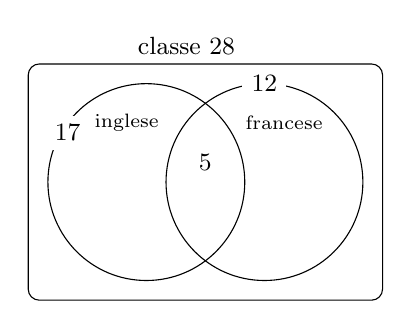
\begin{tikzpicture}[x=5mm, y=5mm,font=\small]

\draw[rounded corners] (-1,-3) rectangle (8,3) (4.5,3)node[above, anchor=south east] {classe 28};
\draw (2,0) circle (2.5);
\draw (5,0) circle (2.5);

\begin{scope}[font=\scriptsize]
\node at (1.5,1.5) {inglese};
\node at (5.5,1.5) {francese};
\end{scope}

\node at (3.5,.5) {5};
\node[fill=white] at (0,1.25) {17};
\node[fill=white] at (5,2.5) {12};
\end{tikzpicture}

\end{center}
\end{multicols}
\end{esempio}

\begin{esempio}
 Il professore di matematica di Piero è piuttosto severo; nella sua classe, di~28 alunni, ha messo solo~6 sufficienze allo scritto e solo~8
all'orale. I ragazzi che sono risultati insufficienti sia allo scritto sia all'orale sono stati~18. Quanti
sono i ragazzi che hanno avuto una votazione sufficiente sia allo scritto che all'orale?

Rappresentiamo la situazione con un diagramma di Eulero-Venn.
\begin{multicols}{2}
$C$ è l'insieme degli alunni della classe di Piero ed è costituito da~28 elementi. $S$ è l'insieme dei ragazzi
sufficienti allo scritto costituito da~6 alunni. $O$ è l'insieme dei ragazzi che sono sufficienti
all'orale ed è costituito da~8 elementi.

Gli elementi di~$\overline{S\cup O}$ sono~18, cioè i ragazzi che
non sono sufficienti né allo scritto, né all'orale.
\begin{center}
 % (c) 2012 Dimitrios Vrettos - d.vrettos@gmail.com
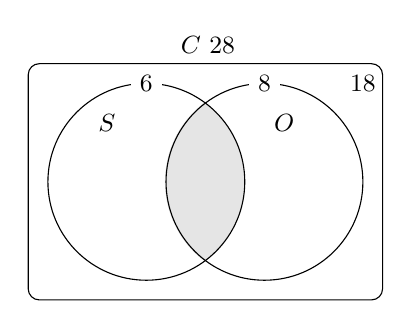
\begin{tikzpicture}[x=5mm, y=5mm,font=\small,filled/.style={fill=circle area, draw=circle edge, thick}]
\def\firstcircle {(2,0) circle (2.5)}
\def\secondcircle{(5,0) circle (2.5)}

\definecolor{circle edge}{gray}{0.9}
\definecolor{circle area}{gray}{0.9}
\draw[rounded corners] (-1,-3) rectangle (8,3) (4.5,3)node[above, anchor=south east] {$C$ 28};
\begin{scope}
\clip \firstcircle;
\fill[filled] \secondcircle;
\end{scope}
\draw\firstcircle;
\draw \secondcircle;

\node at (1,1.5) {$S$};
\node at (5.5,1.5) {$O$};
\node  at (7.5,2.5) {18};

\node[fill=white] at (2,2.5) {6};
\node[fill=white] at (5,2.5) {8};

\end{tikzpicture}

\end{center}
\end{multicols}

L'insieme~$S\cup O$ è quindi costituito da~$28-18=10$ elementi.

Ricordiamo che
\begin{align*}
 &\card(S\cup O)=\card(S)+\card(O)-\card(S\cap O)\\
 \Rightarrow &\card(S\cap O)=\card(S)+\card(O)-\card(S\cup O)\\
 \Rightarrow &\card(S\cap O)=6+8-10=4.
\end{align*}
In conclusione i ragazzi sufficienti allo scritto e all'orale sono~4.
\end{esempio}
\end{exrig}

\ovalbox{\risolvii \ref{ese:7.38}, \ref{ese:7.39}, \ref{ese:7.40}, \ref{ese:7.41}, \ref{ese:7.42}, \ref{ese:7.43}, \ref{ese:7.44}, \ref{ese:7.45}, \ref{ese:7.46}, \ref{ese:7.47},
\ref{ese:7.48}, \ref{ese:7.49}, \ref{ese:7.50}}

\vspazio\ovalbox{\ref{ese:7.51}}
\newpage
 \section{Esercizi}
\subsection{Esercizi dei singoli paragrafi}
\subsubsection*{7.1 - Sottoinsieme}

\begin{esercizio}
\label{ese:7.1}
 Siano~$T=\{t\mid t$ è un triangolo$\}$, $R=\{r\mid r$ è un rettangolo$\}$,
$E=\{e\mid e$ è un triangolo equilatero$\}$. Quale affermazione è vera?
\begin{multicols}{4}
\begin{enumeratea}
\item $R\subset T$;
\item $E\subset T$;
\item $E\subset R$;
\item $T\subset E$.
\end{enumeratea}
\end{multicols}
\end{esercizio}

\subsubsection*{7.2 - Insieme delle parti}
\begin{esercizio}
\label{ese:7.2}
Se~$A=\{x\in\insN\mid 1\le x<3\}$ allora~$\wp (A)$ ha:
\begin{center}
\boxA\quad~2 elementi,\quad\boxB\quad~3 elementi,\quad\boxC\quad~4 elementi,\quad\boxD\quad~8 elementi
\end{center}
\end{esercizio}

\begin{esercizio}
 \label{ese:7.3}
Considera l'insieme~$B=\{x\in\insN\mid 1<x<5\}$
e~$\wp (B)$. Quali delle seguenti affermazioni sono vere o false?
\begin{multicols}{2}
\TabPositions{4cm}
\begin{enumeratea}
 \item $\{1\}\in\wp (B)$ \tab\boxV\quad\boxF
 \item $\emptyset\subset\wp (B)$ \tab\boxV\quad\boxF
 \item $\{\text{2, 5}\}\in\wp (B)$ \tab\boxV\quad\boxF
 \item $\{\emptyset\}\in\wp (B)$ \tab\boxV\quad\boxF
 \item $0\in\emptyset $ \tab\boxV\quad\boxF
 \item $\emptyset\subseteq B$ \tab\boxV\quad\boxF
 \item $\{\text{1, 2, 3}\}\in\wp (B)$ \tab\boxV\quad\boxF
 \item $\{\text{1, 2, 3}\}\notin\wp (B)$ \tab\boxV\quad\boxF
\end{enumeratea}
\end{multicols}
\end{esercizio}

\begin{esercizio}
 \label{ese:7.4}
 Scrivi l'insieme che ha come insieme delle parti
$\{\emptyset\text{, }\{\text{8, 10}\}\text{, }\{8\}\text{, }\{10\}\}$.
\end{esercizio}

\begin{esercizio}
 \label{ese:7.5}
Dato~$H=\{h\mid h$ è una lettera della parola ``MAMMA''$\}$ scrivi
tutti gli elementi di~$\wp (H)$.
\end{esercizio}

\begin{esercizio}
 \label{ese:7.6}
 Dato~$A=\{x\in\insN\mid n<5\text{ e }n\text{ divisore di~12}\}$ scrivi tutti gli elementi di
$\wp (A)$.
\end{esercizio}

\subsubsection*{7.3 - Insieme unione}
\begin{esercizio}
 \label{ese:7.7}
Dati~$A=\{\text{1, 2, 4, 5}\}$ e~$B=\{\text{1, 3, 4, 5, 8}\}$ determina la loro unione dopo
aver rappresentato gli insiemi mediante diagrammi di Eulero-Venn.
 \end{esercizio}

\begin{esercizio}
 \label{ese:7.8}
 Dati gli insiemi~$L=\{\text{1, 2, 5, 6, 7, 8}\}$, $M=\{\text{4, 5, 6, 7, 10}\}$ e~$N=\{\text{2, 3, 5, 7, 9, 10}\}$
determina l'insieme unione completando prima la rappresentazione
grafica poi quella tabulare.
\begin{center}
 % (c) 2012 Dimitrios Vrettos - d.vrettos@gmail.com
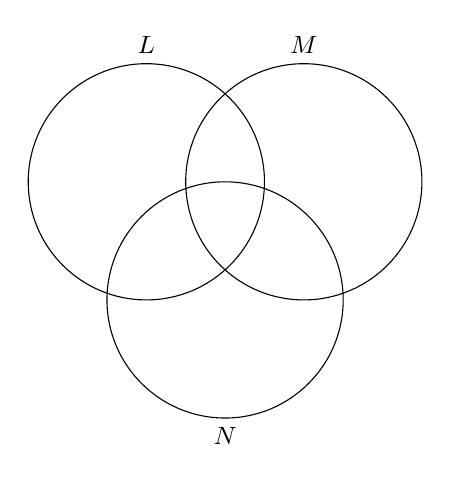
\begin{tikzpicture}[font=\small]
\draw (0,0)circle (1.5) (0,1.5) node[above] {$L$};
\draw(2,0) circle (1.5) (2,1.5) node [above]  {$M$};
\draw(1,-1.5)circle (1.5) (1,-3) node[below]{$N$};
\end{tikzpicture}

\end{center}
\end{esercizio}

\begin{esercizio}
 \label{ese:7.9}
Dati gli insiemi~$C$ delle lettere della parola ``GIARDINO'' e~$D$ delle lettere della
parola ``ORA'', determina la loro unione aiutandoti con la rappresentazione grafica.
 \end{esercizio}

\subsubsection*{7.4 - Insieme intersezione}
 \begin{esercizio}
 \label{ese:7.10}
Dati~$A=\{\text{1, 2, 4, 5}\}$ e~$B=\{\text{1, 3, 4, 5, 8}\}$ determina la loro
intersezione dopo aver rappresentato gli insiemi mediante diagrammi di
Eulero-Venn.
\end{esercizio}

\begin{esercizio}
 \label{ese:7.11}
Dati gli insiemi~$C$ delle lettere della parola ``LIBRO'' e~$D$ delle lettere della
parola ``PASTA'' determina la loro intersezione aiutandoti con la rappresentazione grafica.
\end{esercizio}

\begin{esercizio}
 \label{ese:7.12}
Considerando i~3 insiemi~$S=\{$a, b, c, e, f, s, t$\}$, $T=\{$a, c, g, h, l, s$\}$ e~$U=\{$b, c, d, g, s, t$\}$,
determina l'insieme intersezione dando sia la rappresentazione grafica sia quella tabulare.
 \end{esercizio}

\begin{esercizio}
 \label{ese:7.13}
 Determina l'intersezione tra i seguenti insiemi:
\begin{enumeratea}
 \item $A=\{-3$, $-2$, $-1$, $0$, $+1$, $+2$, $+3\}$, $B=\{-2$, $-1$, $0$, $+1$, $+2$, $+3$, $+4\}$; $A\cap B=\ldots$
 \item $A=\{x\in\insN\mid 2\le x\le~5\}$, $B=\{x\in\insN\mid 3<x<7\}$; $B\cap A=\ldots$
 \item $A=\{x\in\insZ\mid -5\le x\le+5\}$, $B=\{x\in\insZ\mid -15\le x<3\}$; $A\cap B=\ldots$
 \item $A=\{x\in\insN\mid x>100\}$, $B=\{x\in\insN\mid 10<x<20\}$; $B\cap A=\ldots$
 \item $A=\{l$ una lettera di ``SATURNO''$\}$, $B=\{l$ una lettera di ``NETTUNO''$\}$; $A\cap B=\ldots$
\end{enumeratea}
\end{esercizio}

\subsubsection*{7.5 - Insieme differenza}
\begin{esercizio}
\label{ese:7.14}
Dati gli insiemi~$E=\{x\mid x$ è una lettera della parola ``cartellone''$\}$ e
$F=\{x\mid x$ è una lettera della parola ``martello''$\}$, determina
$E-F$ e~$F-E$.
\end{esercizio}

\subsubsection*{7.5 - Insieme complementare}
\begin{esercizio}
\label{ese:7.15}
Verifica, utilizzando la rappresentazione grafica, che
\begin{multicols}{2}
 \begin{enumeratea}
 \item $\overline{A}_{U}\cup A=U$;
 \item $(A-B)\cup (B-A)\cup (\overline{A\cup B})=\overline{A\cap B}$.
 \end{enumeratea}
\end{multicols}
\end{esercizio}

\begin{esercizio}
 \label{ese:7.16}
Dati~$E$ ed~$F$ sottoinsiemi di un insieme~$U$, l'insieme
definito da~$\overline{E\cap F}$ è uguale a:
\begin{center}
\boxA\quad~$E\cup F$\quad\boxB\quad~$\overline{E\cup F}$\quad\boxC\quad~$E\cap F$\quad\boxD\quad~$\overline{E}\cup\overline{F}$
\end{center}
\end{esercizio}

\begin{esercizio}
 \label{ese:7.17}
Dati~$G$ ed~$H$ sottoinsiemi di un insieme~$U$, l'insieme
definito da~$\overline{G\cup H}$ è uguale a:
\begin{center}
\boxA\quad~$\overline{G\cap H}$\quad\boxB\quad~$\overline{G}\cap\overline{H}$\quad\boxC\quad~$\overline{G\cap \overline{H}}$\quad\boxD\quad nessuno dei precedenti
\end{center}
\end{esercizio}

\subsubsection*{7.6 - Leggi di De Morgan}

\begin{esercizio}
 \label{ese:7.18}
 Dimostra la seconda legge di De Morgan, annerendo gli spazi opportuni.
 \begin{center}
 %\usetikzlibrary{decorations.markings}
%\usetikzlibrary{matrix,fit}
%\usetikzlibrary{positioning}
%\usetikzlibrary{shapes.geometric}
%\usetikzlibrary{decorations.pathreplacing}
%\usetikzlibrary{decorations.text}
%\usetikzlibrary{mindmap}
%\usetikzlibrary{plotmarks}
%\usetikzlibrary{backgrounds}
%\usetikzlibrary{patterns}

% (c) 2012 Dimitrios Vrettos - d.vrettos@gmail.com

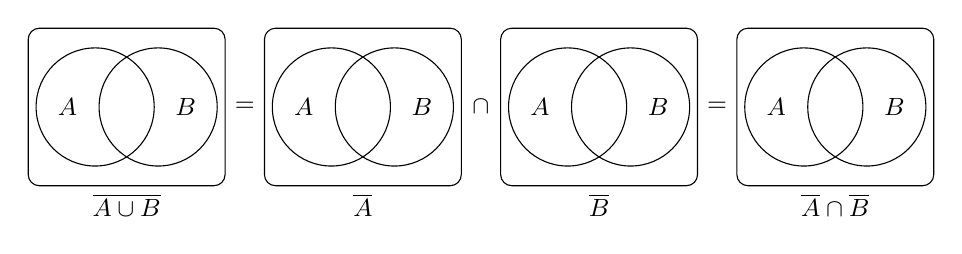
\begin{tikzpicture}[x=5mm,y=5mm,font=\small, outline/.style={draw=circle edge}]
\definecolor{circle area}{gray}{0.9}
\definecolor{circle edge}{rgb}{0,0,0}

\def\firstcircle{(1.7,2) circle (1.5)}
\def\secondcircle{(3.3,2) circle (1.5)}

\begin{scope}[rounded corners]
\foreach \i in {0,6,12,18}
\draw[fill=white] (\i,0) rectangle (\i+5,4);
\end{scope}

\begin{scope}]
\begin{scope}
\clip \firstcircle;
\fill[white] \secondcircle;
\end{scope}
\draw[outline] \firstcircle;
\draw[outline] \secondcircle;
\end{scope}

\begin{scope}[xshift=30mm]
\begin{scope}
\clip \firstcircle;
\fill[white] \firstcircle;
\end{scope}
 \draw[outline]  \firstcircle;
\draw[outline] \secondcircle;
\end{scope}

\begin{scope}[xshift=60mm]
\begin{scope}
\clip \secondcircle;
\fill[white] \secondcircle;
\end{scope}
 \draw[outline]  \firstcircle;
\draw[outline] \secondcircle;
\end{scope}

\begin{scope}[xshift=90mm]
\begin{scope}
\clip \firstcircle;
\fill[white] \secondcircle;
\end{scope}
\draw[outline] \firstcircle;
 \draw[outline] \secondcircle;
\end{scope}

\foreach \x/\xtext in {5.5/$=$,11.5/$\cap$,17.5/$=$}
	\node  at (\x,2) {\xtext};

\foreach \y in {1,7,13,19}
\node  at (\y,2) {$A$};

\foreach \z in {4,10,16,22}
\node  at (\z,2) {$B$};

\foreach \j/\jtext in {2.5/\overline{A\cup B},8.5/\overline{A},14.5/\overline{B},20.5/\overline{A}\cap\overline{B}
}
\node  at (\j,-.5) {$\jtext$};
\end{tikzpicture}



 \end{center}
\end{esercizio}

\subsubsection*{7.7 - Prodotto cartesiano fra insiemi}

\begin{esercizio}
\label{ese:7.19}
Sia~$E=\{x\in\insN\mid 1\le x<3\}$, $F=\{x\mid x$ è una vocale della parola ``TELEFONO''$\}$ e~$G=\{x\in\insN\mid x<-6\}$. Allora:
\begin{enumeratea}
 \item $E=\{1\text{, }\dotfill\}$;
 \item $F=\{\text{e, }\dotfill\}$;
 \item $G=\{\dotfill\}$;
 \item $E\times F=\{(1;\text{e})\text{, }\dotfill\}$;
 \item $F\times E=\{(\text{e};1)\text{, }\dotfill\}$;
 \item $F\times G=\{\dotfill\}$;
 \item $G\times E=\{\dotfill\}$.
\end{enumeratea}
\end{esercizio}

\begin{esercizio}
 \label{ese:7.20}
Quanti sono gli elementi del prodotto cartesiano~$A\times B$, dove~$A$ ha~6 elementi, $B$ ne ha~3:
\begin{center}
 \boxA\quad~9 \quad\boxB\quad~18 \quad\boxC\quad~6 \quad\boxD\quad Non si può sapere.
\end{center}

%\boxA\quad~9 \quad\boxB\quad~18 \quad\boxC\quad~6 \quad\boxD\quad Non si può sapere.
\end{esercizio}


\begin{esercizio}
 \label{ese:7.21}
Sapendo che~$E\times F=\{(\text{x};\text{x})\text{, }(\text{x};\text{y})\text{, }(\text{x};\text{z})\text{, }(\text{y};\text{x})\text{, }(\text{y};\text{y})\text{, }(\text{y};\text{z})\}$, indica gli elementi di~$E$ e di~$F$:
\begin{multicols}{2}
\begin{enumeratea}
 \item $E=\{\dotfill\}$;
 \item $F=\{\dotfill\}$.
\end{enumeratea}
\end{multicols}
\end{esercizio}

\begin{esercizio}
 \label{ese:7.22}
Se~$A\times B$ ha~5 elementi, da quanti elementi possono essere costituiti~$A$ e~$B$?
\begin{center}
 \boxA\quad~1; 5 \quad\boxB\quad~3; 2 \quad\boxC\quad~6; 1 \quad\boxD\quad~2; 3.
\end{center}
\end{esercizio}

\begin{esercizio}
 \label{ese:7.23}
Dati gli insiemi~$A=\{\text{3, 5, 6}\}$ e~$B=\{-2\text{, }1\}$ costruisci il
diagramma cartesiano di~$A\times B$ ed elencane gli elementi.
\end{esercizio}

\begin{esercizio}
 \label{ese:7.24}
 Dato~$A=\{\text{0, 1, 2}\}$ calcola~$A\times A$.
\end{esercizio}

\subsubsection*{7.8 - I diagrammi di Eulero-Venn come modello di un problema}

\begin{esercizio}
\label{ese:7.25}
La scuola ``Step'' organizza corsi di Salsa, Hip Hop e Break Dance.

\begin{enumeratea}
\item Gli iscritti ai corsi sono in tutto~98;
\item 6 frequentano tutti e tre i corsi;
\item 37 frequentano il corso di Salsa;
\item 15 solo i corsi di Salsa e di Hip Hop;
\item 7 solo i corsi Salsa e Break Dance;
\item 9 almeno Hip Hop e Break Dance;
\item 28 Salsa o Break Dance ma non Hip Hop.
\end{enumeratea}

Quanti praticano solo Hip Hop?

Rappresentiamo la situazione con un diagramma di Eulero-Venn.
\begin{center}
 % (c) 2012 Dimitrios Vrettos - d.vrettos@gmail.com
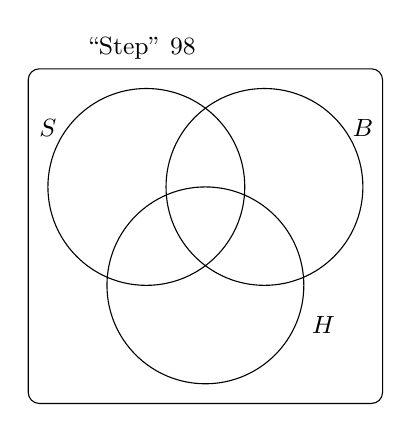
\begin{tikzpicture}[x=5mm, y=5mm,font=\small]

\draw[rounded corners] (0,-5.5) rectangle (9,3) (4.5,3)node[above, anchor=south east] {``Step'' 98};

\draw(3,0) circle (2.5);
\draw(6,0) circle (2.5);
\draw(4.5,-2.5) circle (2.5);

\node at (.5,1.5) {$S$};
\node at (8.5,1.5) {$B$};
\node at (7.5,-3.5) {$H$};

\end{tikzpicture}

\end{center}
$S$ è l'insieme degli iscritti al corso di Salsa, $B$ l'insieme degli iscritti al corso di
Break Dance, $H$ l'insieme degli iscritti al corso di Hip Hop.
\end{esercizio}

\begin{esercizio}
\label{ese:7.26}
Il club ``Argento vivo'' ha~$\np{2500}$ iscritti; nel mese di gennaio ha organizzato alcune
manifestazioni sportive alle quali hanno partecipato~850 degli iscritti
e alcuni tornei di scacchi ai quali hanno partecipato in~780. 320
iscritti al club hanno potuto partecipare, grazie alla perfetta
organizzazione, sia alle manifestazioni sportive sia ai tornei di
scacchi. Quanti soci del club non hanno partecipato a nessuna delle
iniziative e quanti invece hanno partecipato ad almeno una?
\end{esercizio}

\begin{esercizio}[\Ast]
 \label{ese:7.27}
In una scuola di musica si tengono~4 corsi di cui quello di pianoforte è obbligatorio
per tutti i~100 studenti iscritti, mentre quelli di violino, flauto e
chitarra sono facoltativi. Per essere ammessi agli esami di fine anno
bisogna frequentare almeno un corso oltre a quello di pianoforte. Se gli alunni:

\begin{enumeratea}
 \item che frequentano il corso di flauto sono~25 e non frequentano né quello di violino, né quello di chitarra;
 \item iscritti sia al corso di violino sia a quello di chitarra sono~20;
 \item che frequentano il corso di violino sono~46;
 \item che frequentano solo il corso di violino sono tanti quanti quelli che frequentano solo il corso di chitarra.
\end{enumeratea}

Quanti alunni non possono sostenere l'esame finale?
Quale dei seguenti diagrammi di Eulero-Venn può essere preso come modello della situazione?
\begin{center}
 % (c) 2012 Dimitrios Vrettos - d.vrettos@gmail.com

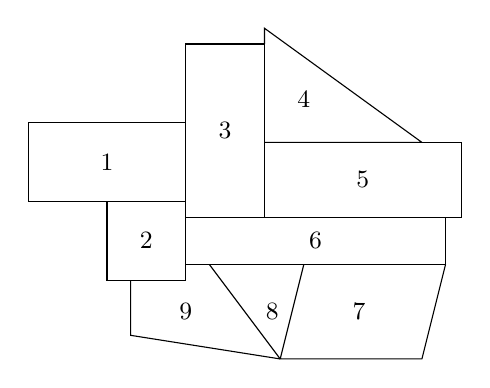
\begin{tikzpicture}[x=10mm,y=10mm, font=\small]
\draw (0,0) rectangle  (2,1) node[midway] {1};
\draw (1,-1) rectangle  (2,0) node[midway] {2};
\draw (2,-.2) rectangle  (3,2) node[midway] {3};
\draw (3,2)-- (3,2.2) -- (5,.75) --(3,.75);
\draw (3,.75) rectangle  (5.5,-.2) node[midway] {5};
\draw (2,-.2) rectangle  (5.3,-.8) node[midway] {6};
\draw (5.3,-.8) -- (5,-2) --(3.2,-2) --(3.5,-.8);
\draw (3.2,-2) -- (2.3,-.8);
\draw (3.2,-2) -- (1.3,-1.7)-- (1.3,-1);
 \node at (3.5,1.3) {4};
 \node at (4.2,-1.4) {7};
 \node at (3.1,-1.4) {8};
 \node at (2,-1.4) {9};
\end{tikzpicture}
\end{center}

\end{esercizio}
\begin{multicols}{2}
\begin{esercizio}[\Ast]
\label{ese:7.28}
I componenti di una compagnia teatrale sanno almeno cantare, ballare,
recitare. Al termine di una rappresentazione si sa che~12 hanno almeno
ballato, 8 hanno almeno cantato e~16 hanno almeno recitato. La
versatilità dei componenti ha permesso che~5 abbiano almeno ballato e
cantato, 3 abbiano almeno cantato e recitato, 8 abbiano ballato e
recitato, 2 ballerini hanno ballato, cantato e recitato. Quanti sono i
componenti della compagnia?
\end{esercizio}

\begin{esercizio}[\Ast]
\label{ese:7.29}
Da un'indagine condotta su consumatori adulti è
risultato che~605 bevono almeno vino, 582 bevono almeno latte, 348
bevono almeno birra, 140 bevono almeno vino e birra, 85 bevono almeno
vino e latte, 56 bevono almeno latte e birra, 25 bevono tutte e tre le
bevande mentre~71 non bevono alcuna delle bevande citate.
\begin{enumeratea}
\item Quante persone bevono una sola bevanda?
\item quante bevono almeno una bevanda?
\item quante sono le persone intervistate?
\end{enumeratea}
\end{esercizio}

\begin{esercizio}[\Ast]
\label{ese:7.30}
In una scuola di lingue sono iscritti~164 studenti; 80 seguono il
corso di francese e~120 il corso di tedesco. Quanti studenti seguono
entrambi i corsi? Quanti studenti seguono
solo il corso di tedesco?
\end{esercizio}

\begin{esercizio}
\label{ese:7.31}
In un classe di~28 allievi, 18 frequentano il laboratorio di teatro,
22 il laboratorio di fotografia, 3 non frequentano alcun laboratorio.
Rappresenta la situazione con un diagramma di Eulero-Venn. Quanto
allievi frequentano entrambi i laboratori? Quanti frequentano almeno un
laboratorio? Quanti non frequentano il laboratorio di teatro?
\end{esercizio}


\begin{esercizio}
\label{ese:7.32}
In una pizzeria, domenica sera, erano presenti~140 persone: 50 hanno
mangiato pizza e calzone, 20 hanno mangiato solo calzone e~15 non hanno
mangiato né pizza né calzone. Il pizzaiolo si chiede se può
conoscere in base alle precedenti informazioni, quante pizze ha
preparato. Aiutalo a risolvere il suo problema illustrando la
situazione con un diagramma di Eulero-Venn, assegnando a ciascun insieme la
sua cardinalità.
\end{esercizio}


\begin{esercizio}
\label{ese:7.33}
In un paese di~$\np{3200}$ abitanti arrivano due quotidiani: il primo è letto da~850
persone, il secondo da~780. Poiché~320 persone leggono entrambi i
quotidiani, quante persone non leggono alcun quotidiano e quante almeno uno?
\end{esercizio}

\begin{esercizio}[Test di ammissione ad Architettura~2008]
\label{ese:7.34}
Nella classe di Asdrubale ci sono~37 allievi. Tutti si sono iscritti
ad almeno una delle due attività extracurriculari (musica e
pallavolo). Alla fine~15 fanno musica e~28 fanno pallavolo.
Quanti allievi, frequentando entrambe le attività, hanno la
necessità di programmare gli orari per evitare sovrapposizioni?
\begin{center}
 \boxA~13\quad\boxB~9\quad\boxC~16\quad\boxD~22\quad\boxE~6
\end{center}
\end{esercizio}



\begin{esercizio}[Test di ammissione a Medicina~2008]
\label{ese:7.35}
In un'aula scolastica, durante la ricreazione, 14
studenti stanno seduti, 8 mangiano la pizza. Con questi dati si può
concludere con certezza che il numero totale~$N$ degli studenti è:
\begin{center}
 \boxA\quad~$N>14$\quad\boxB\quad~$N<14$\quad\boxC\quad~$N>22$\quad\boxD\quad~$N = 22$\quad\boxE\quad~$N\ge~14$
\end{center}
\end{esercizio}


\begin{esercizio}
\label{ese:7.36}
In una scuola di~150 alunni ci sono~23 studenti che frequentano il corso ECDL, 41 studenti che frequentano solo il corso di Inglese, 3
studenti che frequentano tutti e due i corsi. Quanti sono gli studenti che frequentano solo il corso ECDL? Quanti studenti non frequentano
nessuno dei due corsi?
\end{esercizio}

\begin{esercizio}
\label{ese:7.37}
In un giorno di vacanza, 20 alunni dovrebbero studiare latino e
matematica per recuperare le lacune: 8 non studiano latino, 10 studiano
matematica e~4 non studiano niente. Quanti alunni studiano entrambe le
materie?
\end{esercizio}

\begin{esercizio}
\label{ese:7.38}
In una classe di~20 alunni si sta organizzando una gita
scolastica. Durante l'assemblea gli alunni raccolgono
informazioni sulle mete già visitate: 18 hanno visitato Venezia, 14
Roma, 5 Firenze. Solo~3 hanno visitato tutte e tre le città, 5 hanno
visitato Firenze e Venezia, 3 solo Venezia. Quanti hanno visitato solo
Firenze? Quanti hanno visitato Firenze e Roma? Quanti non hanno
visitato nessuna delle tre città? Quanti non hanno visitato Roma?
\end{esercizio}
\end{multicols}
\subsection{Esercizi riepilogativi}

\begin{esercizio}
Siano~$A=\{x\in\insN\mid 1\le x\le~15\}$ e~$B=\{x\in\insN\mid 2\le x\le 20\}$.
\begin{center}
% (c) 2012 Dimitrios Vrettos - d.vrettos@gmail.com
\begin{tikzpicture}[x=3mm, y=5mm,font=\small]

\draw[->, thick] (-1,0)--(24,0) node [above left] {$\insN$};
\draw[pattern =north east lines, pattern color=RedOrange] (1,0) rectangle (15,1) (1,1)node[left] {$A$};
\draw[pattern =north west lines, pattern color=CornflowerBlue] (2,0) rectangle (20,1.5) node[right]{$B$};

\foreach \x/\xtext in {1/1,2/2,15/15,20/20}
\draw[fill] (\x,0)circle (1pt) (\x,0)node [below]{\xtext};
\end{tikzpicture}

\end{center}
Quale delle seguenti affermazioni è vera:
\begin{center}
\boxA\quad~$A\subset B$\quad\boxB\quad~$B\supset A$\quad\boxC\quad$A=B$\quad\boxD\quad$B\not\subset A$
\end{center}
\end{esercizio}

\begin{esercizio}
 Siano~$A=\{x\in\insN\mid x$ è pari e $(1\le x\le 20)\}$ e~$B=\{x\in\insN\mid x$ è multiplo di~6 e $2\le x\le 18\}$.
Quale affermazione è vera?
\begin{center}
 \boxA\quad~$A\subset B$\quad\boxB\quad~$B\supset A$\quad\boxC\quad~$A=B$\quad\boxD\quad~$B\subset A$
\end{center}
\end{esercizio}

\begin{esercizio}
Siano~$A=\{x\in\insN\mid 3\le x\le 10\}$ e~$B=\{x\in\insN\mid 2\le x\le 20\}$.
Quali delle seguenti affermazioni è vera:
\begin{center}
 \boxA\quad~$A\subset B$\quad\boxB\quad~$B\supset A$\quad\boxC\quad~$A=B$\quad\boxD\quad~$B\not\subset A$
\end{center}
\end{esercizio}

\begin{esercizio}
Individua tutti i possibili sottoinsiemi propri formati da tre elementi dell'insieme~$C=\{$a, e, i, o, u$\}$.
\end{esercizio}

\begin{esercizio}
Sia~$A=\{$1, 2, 3, 4$\}$ scrivi i possibili sottoinsiemi propri e impropri di~$A$.
\end{esercizio}

\begin{esercizio}
Associa a ogni diagramma la corretta rappresentazione grafica (ci può essere più di una risposta corretta).

\TabPositions{5cm}
\begin{enumeratea}
 \item $M\subset P$ \tab\boxA\quad\boxB\quad\boxC\quad\boxD\quad\boxE
\item $P\supseteq M$ \tab\boxA\quad\boxB\quad\boxC\quad\boxD\quad\boxE
\item $M\subseteq (M\cup P)$ \tab\boxA\quad\boxB\quad\boxC\quad\boxD\quad\boxE
\item $M\not\subset P$ \tab\boxA\quad\boxB\quad\boxC\quad\boxD\quad\boxE
\item $P\subset (P\cup M)$ \tab\boxA\quad\boxB\quad\boxC\quad\boxD\quad\boxE
\item $M\neq P$ \tab\boxA\quad\boxB\quad\boxC\quad\boxD\quad\boxE
\end{enumeratea}
\begin{center}
% (c) 2012 Dimitrios Vrettos - d.vrettos@gmail.com
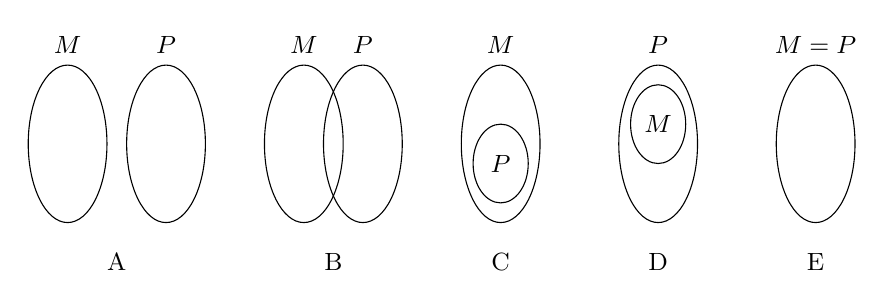
\begin{tikzpicture}[x=5mm, y=5mm,font=\small]

\draw (0,0) ellipse (1 and 2) (0,2.5)node {$M$};
\draw (2.5,0) ellipse (1 and 2)(2.5,2.5) node {$P$};
\node  at (1.25,-3) {A};

\begin{scope}[xshift=30mm]
\draw (0,0) ellipse (1 and 2) (0,2.5)node {$M$};
\draw (1.5,0) ellipse (1 and 2)(1.5,2.5) node {$P$};
\node  at (.75,-3) {B};
\end{scope}

\begin{scope}[xshift=55mm]
\draw (0,0) ellipse (1 and 2) (0,2.5)node {$M$};
\draw (0,-.5) ellipse (.7 and 1) node {$P$};
\node  at (0,-3) {C};
\end{scope}

\begin{scope}[xshift=75mm]
\draw (0,0) ellipse (1 and 2) (0,2.5)node {$P$};
\draw (0,.5) ellipse (.7 and 1) node {$M$};
\node  at (0,-3) {D};
\end{scope}

\begin{scope}[xshift=95mm]
\draw (0,0) ellipse (1 and 2) (0,2.5)node {$M=P$};
\node  at (0,-3) {E};
\end{scope}
\end{tikzpicture}

\end{center}
\end{esercizio}
%\newpage
\begin{esercizio}
Determina l'unione tra i seguenti insiemi:

\begin{enumeratea}
 \item $A=\{-3$, $-2$, $-1$, $0$, $+1$, $+2$, $+3\}$, $B=\{-2$, $-1$, $0$, $+1$, $+2$, $+3$, $+4\}$. $A\cup B=\dotfill$;
 \item $A=\{x\in\insN\mid 2\le x\le 5\}$, $B=\{x\in\insN\mid 3<x<7\}$. $A\cup B=\dotfill$;
 \item $A=\{x\in\insZ\mid -5\le x\le +5\}$, $B=\{x\in\insZ\mid -15\le x<3\}$. $A\cup B=\dotfill$;
 \item $A=\{x\in\insN\mid x>100\}$, $B=\{x\in\insN\mid 10<x<20\}$. $A\cup B=\dotfill$;
 \item $A=\{l$ è una lettera di ``SATURNO''$\}$, $B=\{l$ è una lettera di ``NETTUNO''$\}$. $A\cup B=\dotfill$.
\end{enumeratea}
\end{esercizio}

\begin{esercizio}
Sia~$M_{3}$ l'insieme dei multipli~3 e~$M_{4}$ l'insieme dei multipli di~4, in
generale~$M_{n}$ l'insieme dei multipli del numero~$n$.

 \begin{enumeratea}
 \item Calcola~$M_{3}\cap M_{4}$. Si tratta di~$M\ldots$ l'insieme dei multipli di \ldots;
 \item calcola~$M_{6}\cap M_{4}$. Si tratta di~$M\ldots$ l'insieme dei multipli di \ldots;
 \item calcola~$M_{60}\cap M_{48}$ \ldots;
 \item sai dedurre una regola che, dati due numeri naturali~$m$ e~$n$ calcoli~$M_{m}\cap M_{n}$? Può accadere che questo insieme sia vuoto?
 \end{enumeratea}
\end{esercizio}


\begin{esercizio}
Sia~$D_{4}$ l'insieme dei divisori di~4 e~$D_{6}$ l'insieme dei divisori di~6, in
generale~$D_{n}$ l'insieme dei divisori del numero~$n$.

\begin{enumeratea}
 \item Calcola~$D_{4}\cap D_{6}$. Si tratta di~$D\ldots$ l'insieme dei divisori di \ldots;
 \item calcola~$D_{60}\cap D_{48}$ \ldots;
 \item sai dedurre una regola che, dati due numeri naturali~$m$ e~$n$,
calcoli~$D_{m}\cap D_{n}$? Può accadere che questo insieme sia
vuoto? Qual è il numero minimo di elementi che può contenere?
\end{enumeratea}
\end{esercizio}

\begin{esercizio}
$A=\{x\mid x\in\insQ,0<x<\frac{3}{2}\}$ e~$B=\{x\mid x\in\insQ\text{, }1<x<6\}$, calcola~$A\cap B=\ldots$
\end{esercizio}

\begin{esercizio}
$A=\{x\mid x\in\insQ,-1<x<0\}$ e~$B=\{x\mid x\in\insQ\text{, }\frac{1}{3}<x<6\}$, calcola~$A\cap B=\ldots$
\end{esercizio}

\begin{esercizio}
$A=\{x\mid x\in\insQ,-5<x<10\}$ e~$B=\{x\mid x\in\insQ\text{, }\frac{1}{3}<x<6\}$, calcola~$A\cap B=\ldots$
\end{esercizio}

\begin{esercizio}
$A=\{x\mid x\in\insQ,0\le x<10\}$ e~$B=\{x\mid x\in\insQ\text{, }\frac{1}{3}<x\le~6\}$, calcola~$A\cap B=\ldots$
\end{esercizio}

\begin{esercizio}
Dato l'insieme~$A=\{$3, 4, 5, 6, 7, 8, 9, 12, 32$\}$ e il suo sottoinsieme~$B$ dei multipli di~3, determina gli
insiemi~$A-B$ e~$B-A$.
\end{esercizio}

\begin{esercizio}
Dato l'insieme~$X=\{x\in\insN\mid 10\le x\le~100\}$ e~$Y=\{y\in\insN\mid 10<y<100\}$ determina~$X-Y$ e~$Y-X$.
\end{esercizio}

\begin{esercizio}
Determina la differenza tra i seguenti insiemi:

\begin{esercizio}
Dati gli insiemi~$C$ e~$D$ tali che~$C\subset D$
completa le seguenti relazioni aiutandoti con la rappresentazione
grafica:
\begin{multicols}{3}
\begin{enumeratea}
\item $D-C=\ldots$;
\item $D\cap \overline{C}=\ldots$;
\item $\overline{C\cap D}=\ldots$;
\item $C\cup \overline{C}=\ldots$;
\item $C-D=\ldots$;
\item $C\cap \overline{C}=\ldots$
\end{enumeratea}
\end{multicols}
\end{esercizio}

\begin{enumeratea}
\item $A=\{-3$, $-2$, $-1$, $0$, $+1$, $+2$, $+3\}$, $B=\{-2$, $-1$, $0$, $+1$, $+2$, $+3$, $+4\}$. $A-B=\ldots$;
\item $A=\{x\in\insN\mid 2\le x\le~5\}$, $B=\{x\in\insN\mid 3<x<7\}$. $B-A=\ldots$;
\item $A=\{x\in\insZ\mid -5\le x\le +5\}$, $B=\{x\in\insZ\mid -15\le x<3\}$. $A-B=\ldots$;
\item $A=\{x\in\insN\mid x>100\}$, $B=\{x\in\insN\mid 10<x<20\}$. $B-A=\ldots$;
\item $A=\{l$ è una lettera di ``SATURNO''$\}$, $B=\{l$ è una lettera di ``NETTUNO''$\}$. $A-B=\ldots$
\end{enumeratea}
\end{esercizio}
\pagebreak
\begin{esercizio}
Quale delle seguenti scritture corrisponde a~$\overline{{X\cap \overline{Y}}}$:
\begin{multicols}{4}
 \begin{enumeratea}
 \item $\overline{X}\cup \overline{Y}$
 \item $\overline{X}\cap \overline{Y}$
 \item $\overline{X}\cup Y$
 \item $X\cup \overline{Y}$
 \end{enumeratea}
\end{multicols}
\end{esercizio}


\begin{esercizio}
Esegui le operazioni indicate~$A\cup B$, $A\cap B$, $A-B$.

\begin{enumeratea}
\item $A=\{$2, 4, 6, 8$\}$, $B=\{$1, 3, 6, 9$\}$;
\item $A=\{$a, e, i, o, u$\}$, $B=\{$a, b, c, d, e$\}$;
\item $A=\emptyset$, $B=\{0\}$;
\item $A=\{x\in\insN\mid x$ è pari$\}$, $B=\{x\in\insN\mid x$ è dispari$\}$;
\item $A=\{x\in\insN\mid x$ è multiplo di~2$\}$, $B=\{x\in\insN\mid x$ è multiplo di~4$\}$;
\item $A=\{x\in\insZ\mid -5\le x\le~5\}$, $B=\{x\in\insZ\mid -2\le x\le~8\}$;
\item $A=\{x\in\insN\mid x$ è lettera di ``casa''$\}$, $B=\{x\in\insN\mid x$ è lettera di ``caserma''$\}$.
\end{enumeratea}
\end{esercizio}

\begin{esercizio}
Dato~$A=\{x\in\insN\mid x$ è multiplo di~2$\}$ determina~$\complement_{\insN}A$.
\end{esercizio}

\begin{esercizio}
Dato~$A=\{$I, II, III$\}$ e~$B=\{$a, b$\}$ determina~$A\times B$.
\end{esercizio}

\begin{esercizio}
Dato~$B=\{\text{1, 2, 3}\}$ calcola~$(B\cup B)\cap B$.
\end{esercizio}

\begin{esercizio}
Dati $A=\{$2, 4, 6, 8, 10, 12, 14, 16, 18, 20$\}$, $B=\{$3, 6, 9, 12, 15, 18$\}$ e
$C=\{$1, 3, 5, 7, 9, 11, 13, 15, 17, 19$\}$, calcola
$A\cap B$, $A\cup C$, $(A\cap B)\cup C$, $B\cap C$, $(A\cup B)\cap(B\cup C)$.
\end{esercizio}

\begin{esercizio}
Dati $A=\{x\in\insZ\mid -5\le x<2\}$ e $B=\{x\in\insN\mid -3<x\le~2\}$, calcola
$A\cup B$, $A\cap B$, $B-A$, $\complement_{A}B$, $A\times(A\cap B)$ e~$\wp (B-A)$.
\end{esercizio}

\begin{esercizio}
Per ciascuna delle seguenti affermazioni false dai un controesempio.

\begin{enumeratea}
 \item $A\cup B=A$;
\item $A\cap B=\emptyset\:\Rightarrow\:A=\emptyset $;
\item se~$x$ è multiplo di~2 allora è anche multiplo di~4;
\item se~$\card A =2$ e~$\card B = 5$ allora~$\card A\cup B=7$;
\item se~$\card A =2$ e~$\card B = 5$ allora~$\card A\cap B=2$.
\end{enumeratea}
\end{esercizio}

\begin{esercizio}
In base alla figura rispondi alle domande:
\begin{multicols}{2}
\TabPositions{4.5cm}
\begin{enumeratea}
\item L'insieme~$E$ ha~5 elementi \tab\boxV\quad\boxF
\item $2\in E$ \tab\boxV\quad\boxF
\item $3\notin G$ \tab\boxV\quad\boxF
\item $F\subset G$ \tab\boxV\quad\boxF
\item $F\subset E$ \tab\boxV\quad\boxF
\item $\emptyset \subseteq G$ \tab\boxV\quad\boxF
\item $\card(E)=8$ \tab\boxV\quad\boxF
\item $10\in E$ \tab\boxV\quad\boxF
\item $F\cap E=F$ \tab\boxV\quad\boxF
\item $F\cup G=E$ \tab\boxV\quad\boxF
\item $(E-F)-G=\{\text{1, 4}\}$ \tab\boxV\quad\boxF
\end{enumeratea}
\begin{center}
 % (c) 2012 Dimitrios Vrettos - d.vrettos@gmail.com
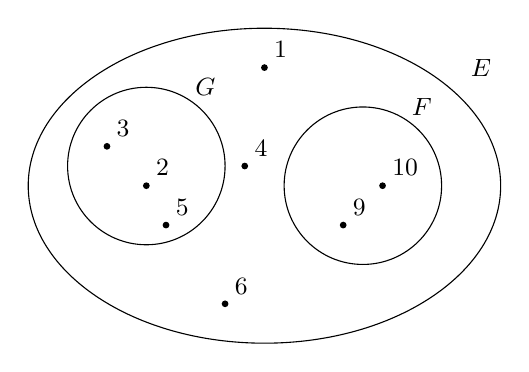
\begin{tikzpicture}[x=5mm, y=5mm,font=\small]

\draw (0,0) ellipse (6 and 4) (5.5,3)node {$E$};
\draw (2.5,0) circle (2)(4,2) node {$F$};
\draw (-3,.5) circle (2)(-1.5,2.5) node {$G$};

\draw[fill](-3,0) circle (1pt ) node[above right]  {2};
\draw[fill](-2.5,-1) circle (1pt ) node[above right]  {5};
\draw[fill](-4,1) circle (1pt ) node[above right]  {3};

\draw[fill](3,0) circle (1pt ) node[above right]  {10};
\draw[fill](2,-1) circle (1pt ) node[above right]  {9};

\draw[fill](0,3) circle (1pt ) node[above right]  {1};
\draw[fill](-.5,.5) circle (1pt ) node[above right]  {4};
\draw[fill](-1,-3) circle (1pt ) node[above right]  {6};
\end{tikzpicture}

\end{center}
\end{multicols}
\end{esercizio}
\pagebreak
\begin{esercizio}
Dato l'insieme~$A=\{$0, 1, 5, 6, 9$\}$ stabilisci
quali dei seguenti sono o meno suoi sottoinsiemi, completando con gli
opportuni simboli le scritture a fianco indicate.
\begin{multicols}{2}
\TabPositions{3cm}
\begin{enumeratea}
\item $B=\{$1, 5, 6$\}$ \tab $B\ldots A$
\item $C=\{$0, 1, 3, 5$\}$ \tab $C \ldots A$
\item $D=\{ \}$ \tab $D \ldots A$
\item $E=\{0\}$ \tab $E \ldots A$
\item $F=\{$5, 6, 7$\}$ \tab $F \ldots A$
\item $G=\{$6, 0, 1, 5, 9$\}$ \tab $G\ldots A$
\end{enumeratea}
\end{multicols}
\end{esercizio}

\begin{esercizio}
Siano dati i seguenti insiemi~$C=\{x\mid x$ è una lettera della parola ``REMARE''\}, $D=\{x\mid x$ è una lettera della parola ``VOLARE''\},
$E=\{x\mid x$ è una lettera della parola ``AMARE''\},
indica quali delle seguenti relazioni sono vere:
\begin{center}
\boxA\quad~$D\subseteq C$\quad\boxB\quad~$D\not\subset E$\quad\boxC\quad~$C=E$\quad\boxD\quad~$E\supseteq C$
\end{center}
\end{esercizio}

\begin{esercizio}
Completa la seguente tabella:

\begin{tabular*}{.9\textwidth}{@{\extracolsep{\fill}}*{2}{cl}}
\toprule
Simbologia & Significato\\
\midrule
$A=\{a\text{, }b\text{, }c\text{, }d\}$ & $A$ è formato dagli \dotfill~$a\text{, }b\text{, }c\text{, }d$.\\
$a\in A$ & L'elemento~$a$ \dotfill all'insieme~$A$.\\
\dotfill & L'elemento f non appartiene all'insieme~$A$.\\
$B\subset A$ & L'insieme~$B$ è \ldots\ldots nell'insieme~$A$, ovvero~$B$ è un \ldots\ldots di~$A$.\\
\dotfill & L'insieme vuoto è un sottoinsieme di~$A$.\\
\dotfill & L'insieme~$C$ è l'unione degli insiemi~$A$ e~$B$.\\
$D=A\cap B$ & L'insieme~$D$ è \dotfill degli insiemi~$A$ e~$B$.\\
$A\cap F=\emptyset $& $A$ e~$F$ sono insiemi \dotfill cioè non hanno \dotfill \\
$L=\complement_{A}B$ & L'insieme~$L$ è \dotfill \\
\dotfill & L'insieme~$M$ è la differenza tra~$A$ e~$B$.\\
\bottomrule
\end{tabular*}
\end{esercizio}

\begin{esercizio}
Rappresenta graficamente l'insieme~$A=\{x\in\insN\mid x\le 25$ e $x$ è pari$\}$ e
$B=\{x\in\insN\mid x\le 27$ e $x$ è multiplo di~4$\}$ e stabilisci se~$A\supseteq B$.
\end{esercizio}

\begin{esercizio}
Verifica usando i diagrammi di Eulero-Venn che se~$A\subset B$ e~$B\subset C$ allora~$A\subset C$. Le relazioni valgono
anche se il simbolo~``${\subset}''$ viene sostituito con~``${\subseteq}''$?
\end{esercizio}

\begin{esercizio}
Dato~$A=\{\text{do, re, mi}\}$ determina l'insieme delle parti~$\wp (A)$.
\end{esercizio}

\begin{esercizio}
Considerato l'insieme~$X=\{\text{a, c, d, t, o}\}$ stabilisci se le seguenti affermazioni sono vere o false.

\TabPositions{8cm}
\begin{enumeratea}
\item $\{x\mid x\text{ è una vocale della parola ``carota''}\} \subset X$ \tab\boxV\quad\boxF
\item $\{\text{a, t}\}\not\subset \wp (X)$ \tab\boxV\quad\boxF
\item $\{\text{a, t}\}\in \wp (X)$ \tab\boxV\quad\boxF
\item $0\in X$ \tab\boxV\quad\boxF
\item $\emptyset \in \wp (X)$ \tab\boxV\quad\boxF
\item $X\in \wp (X)$ \tab\boxV\quad\boxF
\end{enumeratea}
\end{esercizio}

\pagebreak
\begin{esercizio}
Se~$U$ è l'insieme universo degli italiani, $D$ l'insieme delle donne italiane,
$L$ l'insieme degli italiani laureati, $S$ l'insieme degli italiani sposati, cosa rappresentano
i seguenti insiemi?
\begin{multicols}{3}
\begin{enumeratea}
\item $\overline{D}$;
\item $L\cap D$;
\item $\overline{{L\cup D\cup S}}$;
\item $L-S$;
\item $\overline{{L}}\cap S$;
\item $\overline{{L\cap D\cap S}}$.
\end{enumeratea}
\end{multicols}
\end{esercizio}


\begin{esercizio}
Quanti elementi ha~$\wp (H)$ sapendo che $H$ ha~7 elementi?
\begin{center}
 \boxA\quad~49\quad\boxB\quad~64\quad\boxC\quad~128\quad\boxD\quad~7\quad\boxE\quad14
\end{center}
\end{esercizio}

\begin{esercizio}
Scrivi l'insieme che ha per insieme delle parti:
$\{\emptyset\text{, }\{\text{Mauro}\}\text{, }\{\text{Mario}\}\text{, }\{\text{Mauro, Mario}\}\}$.
\end{esercizio}

\begin{esercizio}
Se~$A\cup B=B$ cosa puoi dire di~$A$ e~$B$?
\begin{center}
 \boxA\quad~$B\subseteq A$\quad\boxB\quad~$A\notin B$\quad\boxC\quad~$A\subseteq B$\quad\boxD\quad~$A\subset B$\quad\boxE\quad$A\cap B=\emptyset $
\end{center}
\end{esercizio}

\begin{esercizio}
Dati gli insiemi~$A=\{\text{10, 20, 30, 40, 50}\}$ e $B=\{\text{20, 30, 50}\}$,
determina un insieme~$C$ tale che:
\begin{multicols}{4}
\begin{enumeratea}
 \item $B\cup C=A$;
 \item $A\cap C=B$;
 \item $C\cup C=B$;
 \item $C\cap C=A$.
\end{enumeratea}
\end{multicols}
\end{esercizio}

\begin{esercizio}
Dati gli insiemi~$A=\{x\in\insN\mid x\le 10$ e $x$ è pari$\}$,
$B=\{x\in\insN\mid x\le 20$ e $x$ è divisibile per~4$\}$ e
$C=\{$1, 2$\}$, determina~$(A\cap B)\times C$.
\end{esercizio}

\begin{esercizio}
Dimostra la proprietà distributiva dell'intersezione rispetto l'unione annerendo gli spazi opportuni.
\begin{center}
 % (c) 2012 Dimitrios Vrettos - d.vrettos@gmail.com
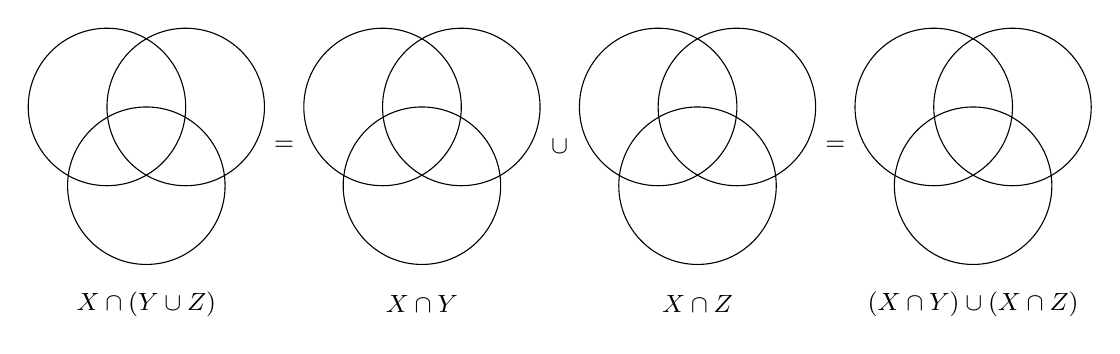
\begin{tikzpicture}[x=5mm, y=5mm,font=\small]

\draw (0,0) circle (2);
\draw (2,0) circle (2);
\draw (1,-2) circle (2);

\begin{scope}[xshift=35mm]
\draw (0,0) circle (2);
\draw (2,0) circle (2);
\draw (1,-2) circle (2);
\end{scope}

\begin{scope}[xshift=70mm]
\draw (0,0) circle (2);
\draw (2,0) circle (2);
\draw (1,-2) circle (2);
\end{scope}

\begin{scope}[xshift=105mm]
\draw (0,0) circle (2);
\draw (2,0) circle (2);
\draw (1,-2) circle (2);
\end{scope}

\foreach \x/\xtext in {4.5/=,11.5/\cup,18.5/=}
\node  at (\x,-1) {$\xtext$};

\foreach \xi/\xitext in {1/$X\cap(Y\cup Z)$,8/$X\cap Y$,15/$X\cap Z$,22/$(X\cap Y)\cup(X\cap Z)$}
\node  at (\xi,-5) {\xitext};
\end{tikzpicture}

\end{center}

\end{esercizio}

\begin{esercizio}
Se~$E-F=E$ cosa puoi dire di~$E$ e~$F$?
\begin{center}
 \boxA\quad~$E\cup F=E$\quad\boxB\quad~$E=F$\quad\boxC\quad~$E\subseteq F$\quad\boxD\quad~$F\subset E$\quad\boxE\quad~$E\cap F=\emptyset $
\end{center}
\end{esercizio}

\begin{esercizio}
Dimostra la proprietà distributiva dell'unione rispetto l'intersezione annerendo gli spazi opportuni
e inserendo le formule opportune.
\begin{center}
 % (c) 2012 Dimitrios Vrettos - d.vrettos@gmail.com
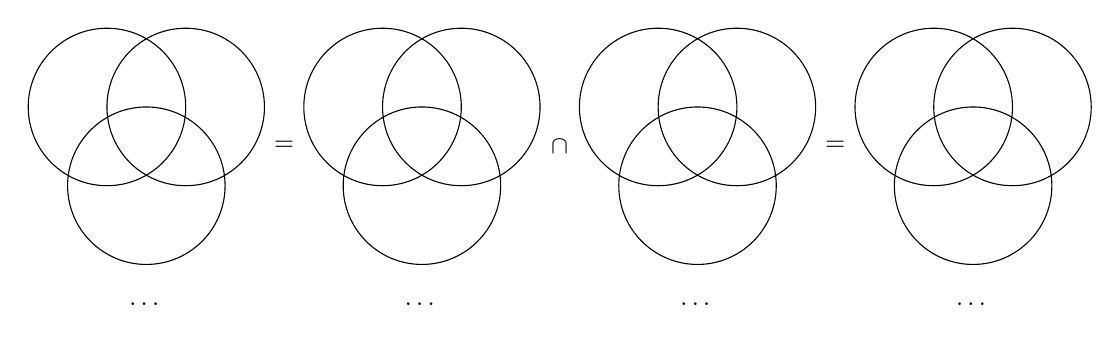
\begin{tikzpicture}[x=5mm, y=5mm,font=\small]

\draw (0,0) circle (2);
\draw (2,0) circle (2);
\draw (1,-2) circle (2);

\begin{scope}[xshift=35mm]
\draw (0,0) circle (2);
\draw (2,0) circle (2);
\draw (1,-2) circle (2);
\end{scope}

\begin{scope}[xshift=70mm]
\draw (0,0) circle (2);
\draw (2,0) circle (2);
\draw (1,-2) circle (2);
\end{scope}

\begin{scope}[xshift=105mm]
\draw (0,0) circle (2);
\draw (2,0) circle (2);
\draw (1,-2) circle (2);
\end{scope}

\foreach \x/\xtext in {4.5/=,11.5/\cap,18.5/=}
\node  at (\x,-1) {$\xtext$};

\foreach \xi in {1,8,15,22}
\node  at (\xi,-5) {\ldots};
\end{tikzpicture}

\end{center}
\end{esercizio}
%\newpage
\begin{esercizio}
Dati i seguenti insiemi~$A=\{x\in\insN\mid x\le~25\}$, $B=\{x\in\insN\mid 4<x\le~9\}$, $C=\{x\in\insN\mid x<25\}$ e~$D=\{x\in\insN\mid x>7\}$.
Scegli fra i seguenti i loro complementari.
\begin{multicols}{2}
\begin{enumeratea}
\item $E=\{x\in\insN\mid x\ge~25\}$;
\item $F=\{x\in\insN\mid x\le~6\}$;
\item $G=\{x\in\insN\mid x>25\}$;
\item $H=\{x\in\insN\mid x<7\}$;
\item $I=\{x\in\insN\mid x<4\text{ e }x\ge~8\}$;
\item $L=\{x\in\insN\mid x<4\text{ o }x\ge~10\}$;
\item $M=\{x\in\insN\mid x\le~4\text{ e }x\ge~9\}$.
\end{enumeratea}
\end{multicols}
\end{esercizio}

\begin{esercizio}
Quali dei seguenti sono sottoinsiemi dei numeri pari? L'insieme dei

\begin{center}
 \boxA\quad multipli di~4\quad\boxB\quad multipli di~3\quad\boxC\quad multipli di~6\quad\boxD\quad numeri primi
\end{center}
\end{esercizio}

\begin{esercizio}[\Ast]
In una classe di~30 allievi~16 hanno debito in matematica, 20 in
italiano, 10 non hanno avuto nessun debito. Rappresenta la situazione
con un diagramma di Eulero-Venn.

\begin{enumeratea}
\item quanti allievi hanno debito in entrambe le materie;
\item quanti allievi hanno almeno un debito;
\item quanti allievi non hanno debito in italiano;
\item quanti allievi non hanno debito in matematica.
\end{enumeratea}
\end{esercizio}

\begin{esercizio}
Quali dei seguenti insiemi possono essere sottoinsiemi dell'insieme dei quadrilateri?
L'insieme dei:
\begin{multicols}{3}
\begin{enumeratea}
 \item quadrati;
 \item rombi;
 \item trapezi;
 \item triangoli equilateri;
 \item poligoni;
 \item cerchi;
 \item parallelogrammi.
\end{enumeratea}
\end{multicols}
\end{esercizio}


\begin{esercizio}
Dati gli insiemi~$A=\{x\mid x\in\insN$, $x<10\}$, $B=\{x\mid x\in\insN$, $5<x\le 16\}$ e
$C=\{x\mid x\in\insN$, $x\ge~7\}$ determina:
\begin{multicols}{4}
\begin{enumeratea}
\item $A\cup B\cup C$;
\item $A\cap B\cap C$;
\item $(A\cup B)\cap C$;
\item $(B\cap C)\cup A$.
\end{enumeratea}
\end{multicols}
\end{esercizio}


\begin{esercizio}
Dato~$A = \{x\mid x$ è un numero naturale, $x$ è pari e $x>12\}$ determina l'insieme complementare di~$A$.
\end{esercizio}

\begin{esercizio}
Quanti sono i sottoinsiemi dell'insieme che contiene come elemento
l'insieme vuoto?
\end{esercizio}

\begin{esercizio}
Dati $A=\{x\mid x$ è divisore di~12$\}$, $B=\{x\mid x$ è divisore di~6$\}$ e
$C=\{x\mid x$ è divisore di~15$\}$, determina:
\begin{multicols}{4}
 \begin{enumeratea}
 \item $A\cup B$;
 \item $A\cup C$;
 \item $A\cup B\cup C$;
 \item $A\cap B$;
 \item $B\cap C$;
 \item $A\cap C$;
 \item $A\cap B\cap C$;
 \item $A\cap(B\cup C)$.
 \end{enumeratea}
\end{multicols}
\end{esercizio}


\begin{esercizio}
Dato l'insieme~$U=\{x\mid x=2n+1$, $n\in\insN$, $0\le n\le~5\}$:

\begin{enumeratea}
\item rappresenta~$U$ in forma tabulare;
\item costruisci due sottoinsiemi propri~$A$ e~$B$ di~$U$ tali che~$A\cap B=\emptyset $;
\item determina~$A\cup B$ e~$A-B$, dai il risultato con rappresentazione tabulare e mediante diagrammi di
Eulero-Venn.
\end{enumeratea}
\end{esercizio}
\pagebreak
\begin{esercizio}
In base agli insiemi rappresentati con il diagramma di Eulero-Venn nella figura determina gli insiemi richiesti:
\begin{multicols}{2}
\begin{enumeratea}
\item $A\cup B$;
\item $\overline{A\cup B\cup C}$;
\item $A\cap B$;
\item $B\cap C$;
\item $A\cap B\cap C$;
\item $A\cap (B\cup C)$;
\item $A\cup (B\cap C)$;
\item $B\cap \overline{C}$;
\item $(A\cup B)-C$;
\item $B\cap \overline{C}$
\item $C-(A\cap B)$;
\item $\overline{(A\cup B)}-C$.
\end{enumeratea}
\begin{center}
 % (c) 2012 Dimitrios Vrettos - d.vrettos@gmail.com
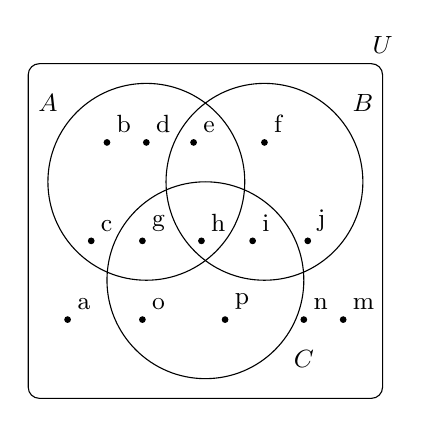
\begin{tikzpicture}[x=5mm, y=5mm,font=\small]

\draw[rounded corners] (-4,-5.5) rectangle (5,3) node[above] {$U$};
\draw (-1,0) circle (2.5) (-3.5,2)node {$A$};
\draw (2,0) circle (2.5) (4.5,2)node {$B$};
\draw (0.5,-2.5) circle (2.5) (3,-4.5)node {$C$};

\foreach \x/\xtext in {-2/b,-1/d,0.2/e,2/f}
\draw[fill] (\x,1)circle(1pt) node[above right]{\xtext};

\foreach \x/\xtext in {-2.4/c,-1.1/g,0.4/h,1.7/i, 3.1/j}
\draw[fill] (\x,-1.5)circle(1pt) node[above right]{\xtext};

\foreach \x/\xtext in {-3/a,-1.1/o,1/p,3/n, 4/m}
\draw[fill] (\x,-3.5)circle(1pt) node[above right]{\xtext};
\end{tikzpicture}

\end{center}
\end{multicols}
\end{esercizio}


\begin{esercizio}
Determina l'insieme~$\wp(A)$, insieme delle parti di~$A$, dove $A$ è l'insieme delle lettere della parola ``NONNA''.
\end{esercizio}

\begin{esercizio}
Nel seguente diagramma di Eulero-Venn gli insiemi~$r$, $s$, $t$
sono rette, gli elementi~$A$, $B$, $C$, $D$ sono punti. Dai una
rappresentazione geometrica, individuando le rette e che corrispondono
alla seguente situazione.

\begin{center}
 % (c) 2012 Dimitrios Vrettos - d.vrettos@gmail.com
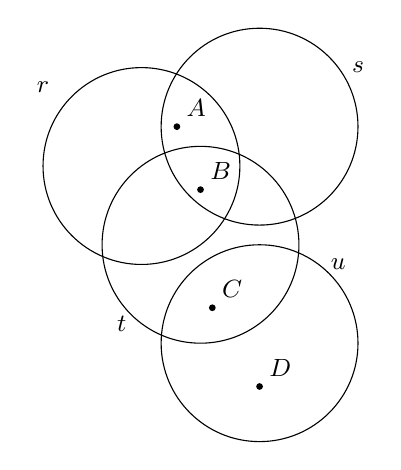
\begin{tikzpicture}[x=5mm, y=5mm,font=\small]
\draw (-1,0) circle (2.5) (-3.5,2)node {$r$};
\draw (2,1) circle (2.5) (4.5,2.5)node {$s$};
\draw (0.5,-2) circle (2.5) (-1.5,-4)node {$t$};
\draw (2,-4.5) circle (2.5) (4,-2.5)node {$u$};

\draw[fill] (-.1,1) circle (1pt) node[above right]  {$A$};
\draw[fill] (.5,-.6) circle (1pt) node[above right]  {$B$};
\draw[fill] (.8,-3.6) circle (1pt) node[above right]  {$C$};
\draw[fill] (2,-5.6) circle (1pt) node[above right]  {$D$};
\end{tikzpicture}

\end{center}
\end{esercizio}

\subsection{Risposte}

\paragraph{7.27.} 3; A.

\paragraph{7.28.} 22.

\paragraph{7.29.} a)~$\np{1048}$,\quad b)~$\np{1279}$,\quad c)~$\np{1350}$.

\paragraph{7.30.} 36; 84.

\paragraph{7.84.} a)~16,\quad b)~20,\quad c)~10,\quad d)~14.


\cleardoublepage
